%!TEX root = thesis.tex
\chapter{Results and Discussion}
\label{ch:results}

With the fully functional parametric model, various aspects of dynamic PV shading systems were evaluated for the ASF case study. This chapter presents and discusses the results of these evaluations. First, the base case is evaluated, visualizing the optimisation and the main outputs of the parametric model. Next, the influence of the angle actuation is discussed and the optimisation for PV electricity output is compared to an approach using sun-tracking. This is followed by sensitivity evaluations on the building orientation, the building location, and various building system parameters. Finally, the influence of different combination settings is shown and the potential of independent actuation is evaluated. 
%Optimum angles and their corresponding electricity use were found for the building energy simulation for all hours of the year. For the radiation and PV evaluations, a grid-convergence study was performed and results of an optimising angle strategy was compared to sun-tracking. The combined simulations could then be evaluated to find the most efficient overall combinations and the sensitivities of various parameters on the system performance was found.

%\section{Combined Evaluation}

\section{Base Case Evaluation}
\label{s:baseCase}
	By combining results for building energy simulations and PV electricity production, the overall optimum configurations can be found. Figures \ref{fig:monthly_altitude} and \ref{fig:monthly_azimuth} detail carpet-plots of the facade optimised to maximise PV generation, and minimise heating, cooling and lighting demands independently. The simulation was done for a base case with a total of 49 angle combinations with seven different states for the altitude and the azimuth angles, i.e. a step size of $15\degree$. For simplicity, the altitude angles are presented separately to the azimuth angles in Figure \ref{fig:monthly_altitude} and Figure \ref{fig:monthly_azimuth}, respectively.  %While the altitude angles are shown in Figure \ref{fig:monthly_altitude}, the corresponding azimuth angles of the same optimisation are shown in Figure \ref{fig:monthly_azimuth}.

	\begin{figure*}
		\begin{center}
		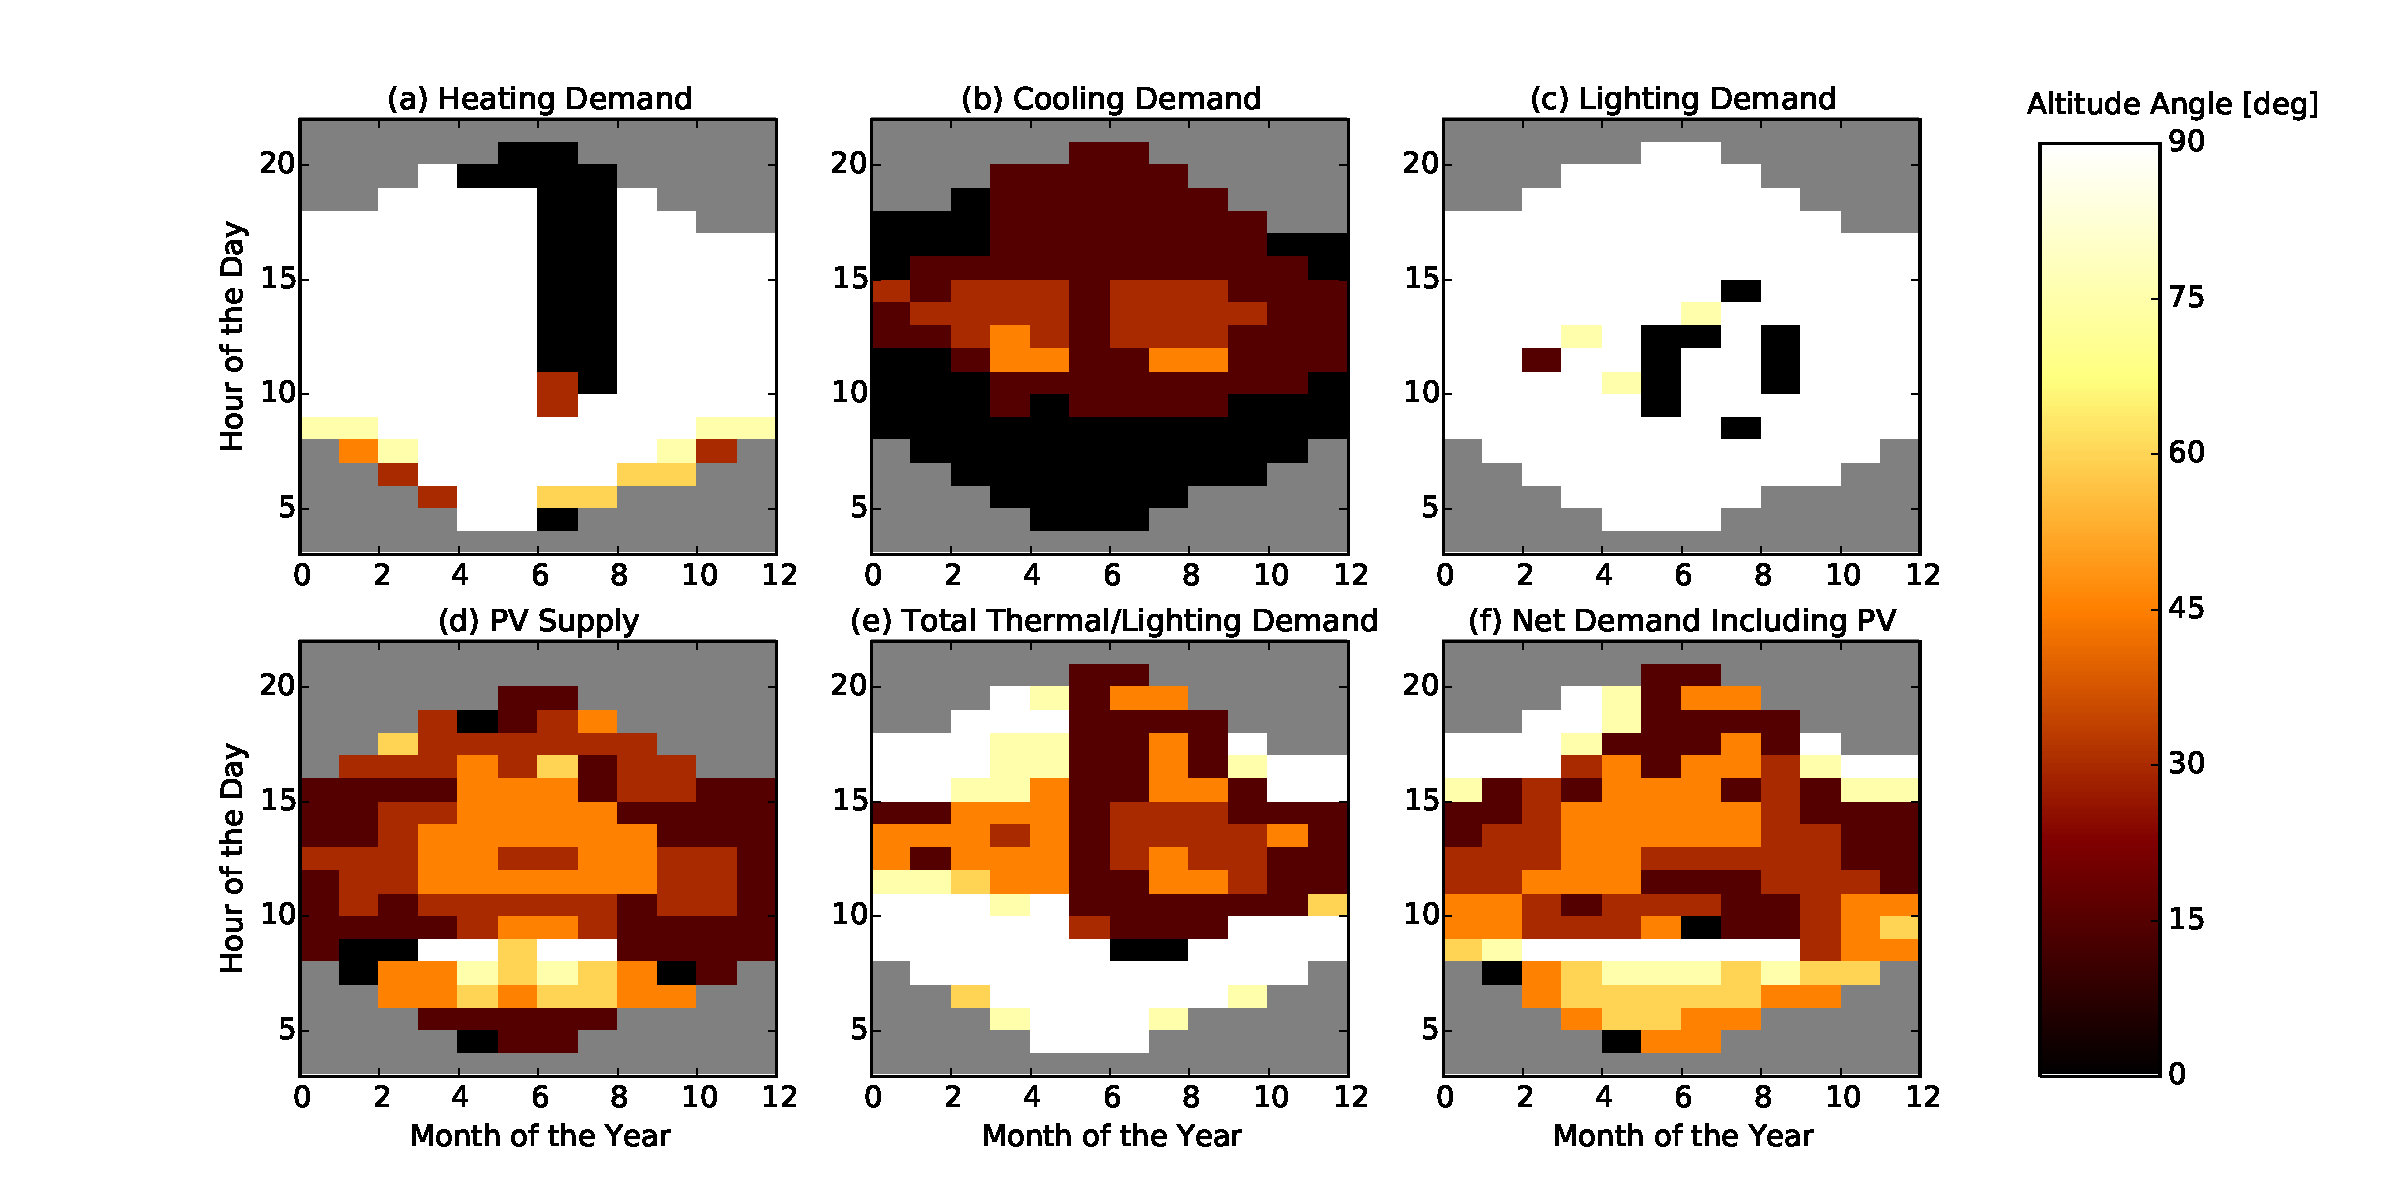
\includegraphics[width=\textwidth, trim= 1cm 0.5cm 1cm 1.4cm,clip]{monthly_altitude}
		\caption{Carpet plots detailing the optimal altitude angles to minimise the (a) heating demand, (b) cooling demand, (c) lighting demand, and (d) maximise PV electricity production. Figure (e) details the combinations for optimum building thermal management without PV production, (f) also includes the PV production. Small angles correspond to closed positions, whereas large angles represent open positions. The corresponding azimuth angles for each hour can be seen in the following Figure (\ref{fig:monthly_azimuth}).}
		\label{fig:monthly_altitude}
		\end{center}
	\end{figure*}

	\begin{figure*}
		\begin{center}
		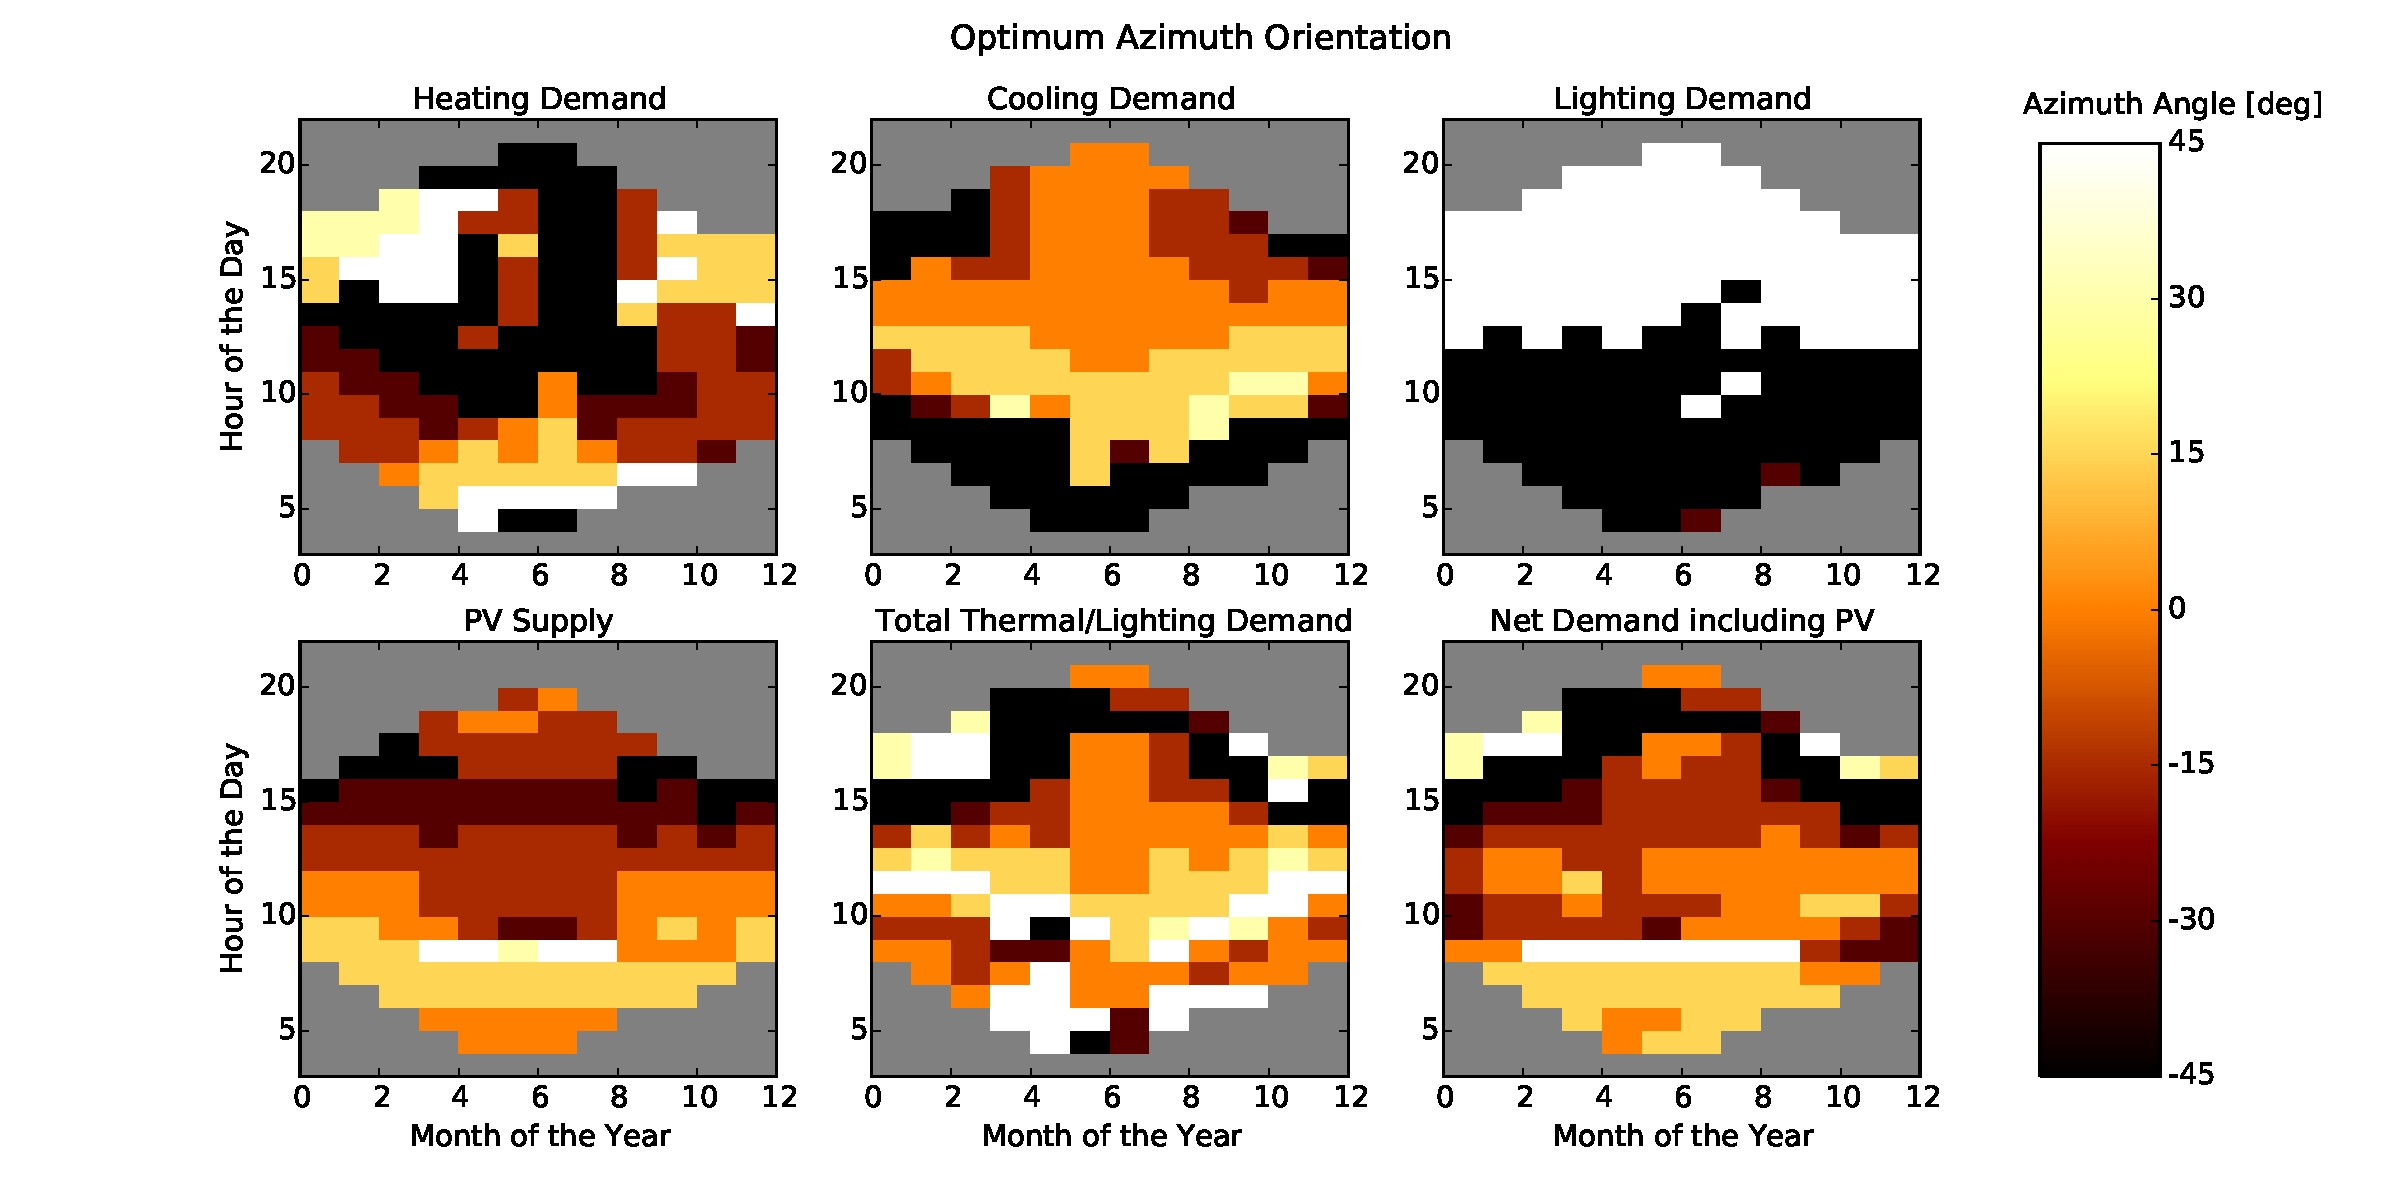
\includegraphics[width=\textwidth, trim= 1cm 0.5cm 1cm 1.4cm,clip]{monthly_azimuth}
		\caption{Carpet plots detailing the optimal azimuth angles to minimise the (a) heating demand, (b) cooling demand, (c) lighting demand, and (d) maximise PV electricity production. Figure (e) details the combinations for optimum building thermal management without PV production, (f) also includes the PV production. Negative angles correspond to the panels facing west, whereas positive angles represent east-facing panels. The corresponding altitude angles for each hour can be seen in the previous Figure (\ref{fig:monthly_altitude}).}
		\label{fig:monthly_azimuth}
		\end{center}
	\end{figure*}

	In the altitude angle visualization it can be seen how open configurations (light coloured) are chosen to minimise the building heating (Fig. \ref{fig:monthly_altitude}a) and lighting (Fig. \ref{fig:monthly_altitude}c) demand. Likewise, closed configurations (dark colours) are the preferred solutions to minimise the cooling demand (Fig. \ref{fig:monthly_altitude}b). The PV optimisation tends to choose more open angles, corresponding to the minimisation of longitudinal shading as will be described in Section \ref{s:compareSunTracking}. In Figure \ref{fig:monthly_altitude}e, the angles that optimise the overall building demand are shown. The optimisation chooses open positions at hours where heating and lighting are important, whereas closed positions are used for hours where cooling is dominant. The configurations for total energy minimisation - including the PV electricity production - are depicted in Figure \ref{fig:monthly_altitude}f. It can be seen that there is a conflict in the summer evenings between minimising lighting and cooling demands. Likewise, there is a conflict between heating and PV production during the winter months. The overall energy optimisation shows a strong tendency to follow the optimal PV production pattern. This, however, changes if the building system becomes more inefficient. Less efficient heating, for example, would result in configurations optimised for heating overpowering those of PV electricity generation.

	Similar patterns can be seen for the azimuth variations (Fig. \ref{fig:monthly_azimuth}). The azimuth angles correspond to the deviation from the building facade normal. As described in Section \ref{s:caseStudy}, the simulation was done for a south-facing facade. This means an angle with a positive sign represents the panels facing towards south-east (bright colours), whereas negative angles represent the panels facing towards south-west (dark colours). It can be seen that for heating and lighting, the facade takes positions that let the sun in, whereas for cooling the facade follows a sun-tracking pattern which prevents radiation from entering the room. The PV optimisation also follows a sun-tracking pattern, though with a deviation towards facing east. This is caused by the PV-layout and the effects of longitudinal shading \cite{hofer2016}. The optimisation minimises longitudinal shading in order to maximise PV electricity production. 

	\begin{figure*}[b!!]
		\begin{center}
		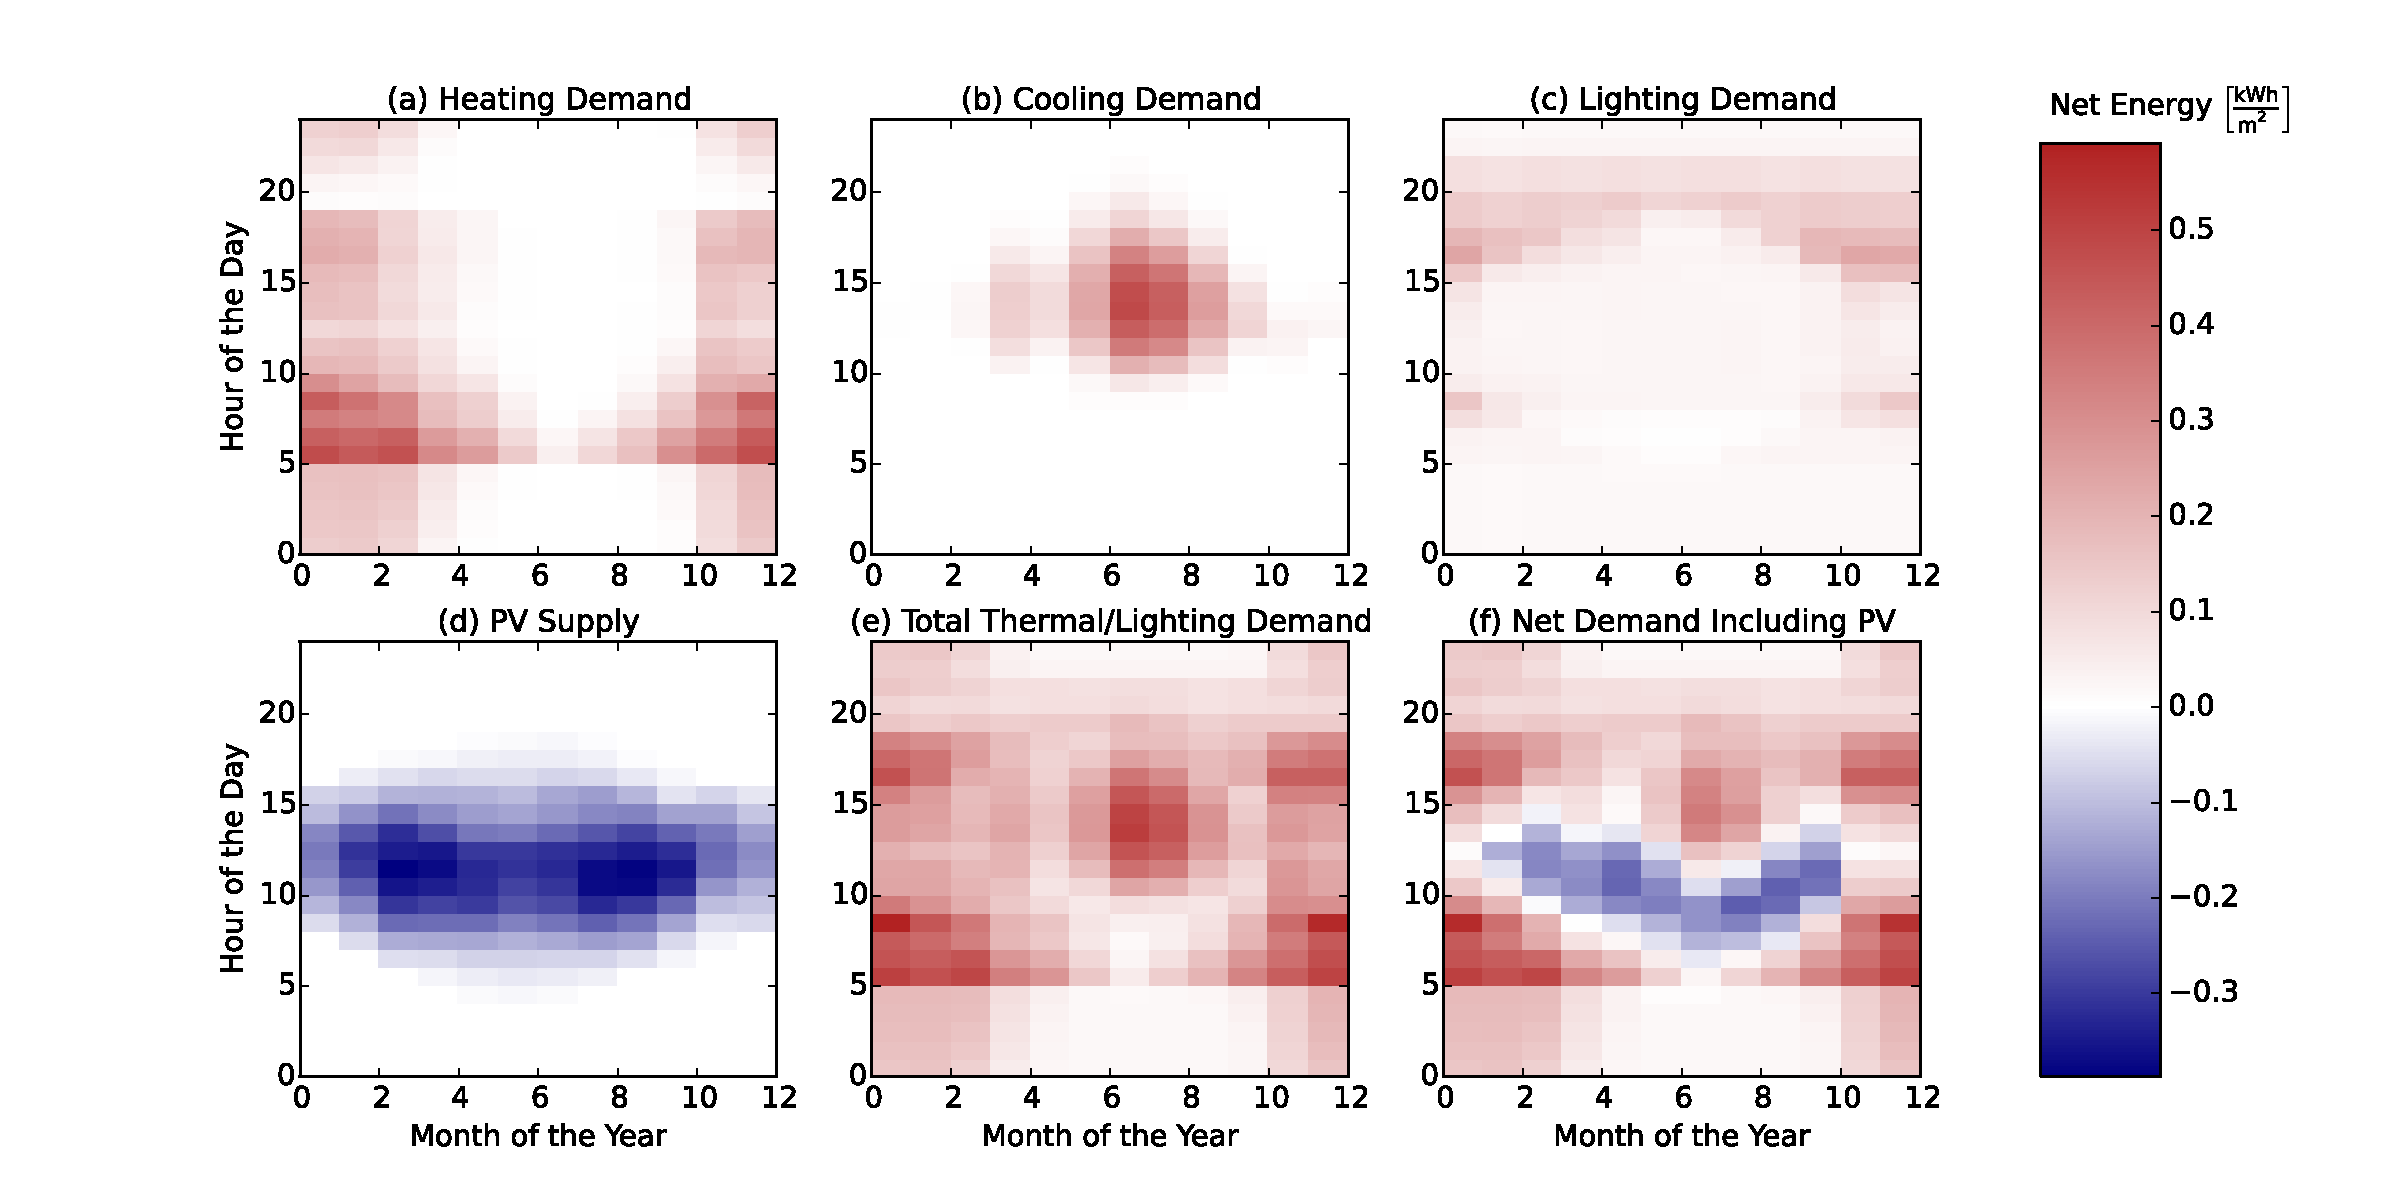
\includegraphics[width=\textwidth, trim= 1cm 0.5cm 1cm 1.4cm,clip]{monthly_energy_perArea}
		\caption{Carpet plots detailing the net energy consumption. Each square represents the total energy consumption for that specific hour of the entire month. Red colours detail the energy demand, while blue colours detail the energy supply.}
		\label{fig:carpetplot_energy}
		\end{center}
	\end{figure*}

	Figure \ref{fig:carpetplot_energy} shows the net energy use at these optimum angles. (a) shows that heating is mainly dominant in the winter and in the mornings, cooling (b) is primarily needed in the summer afternoons, lighting (c) at hours of low or no solar insolation, whereas PV electricity production (d) is dominant at hours with high solar insolation. (e) shows the total building energy demand and (f) visualizes the net energy demand including the PV electricity production. It can be seen that there is a net negative energy demand for most sunlit hours, meaning that the ASF is generating more energy than is used by the building for these hours. 

	Overall, the optimization yields an energy benefit of 9\% compared to the best performing fixed solar facade solution, and the PV electricity production is able to compensate for 41\% of the total building energy demand. Further visualisations of the building energy demand and the corresponding optimum positions can be found in Appendix \ref{s:buildingResults}. 

	


\section{Influence of Angle Actuation}
\label{s:actuation}
	In order to analyse the influence of the actuation, three-dimensional plots can be used to display all evaluated configurations and their corresponding energy benefit. In Figure \ref{fig:3d}, the energy benefits of the altitude actuation are visualized for the months of March (a), June (b) and September (c). Each plot displays one cumulative day in hourly resolution. The x-axis  represents the altitude angles (19 different angles were evaluated with a step size of $5\degree$), the y-axis corresponds to the hour of the day, and the z-axis represents the energy benefit of the actuation, i.e. the difference in energy usage between the evaluated angle and the angle that yields the worst overall energy usage for each hour. It can be seen that the energy benefit is by far the largest around noon. Furthermore, positions that are rather closed tend to have the highest influence for the said mid-day hours. Open positions normally yield the worst benefits, except for some early morning or evening hours, where heating and lighting become important. 

	%\newpage

	\begin{figure*}[h!]
		\begin{center}
		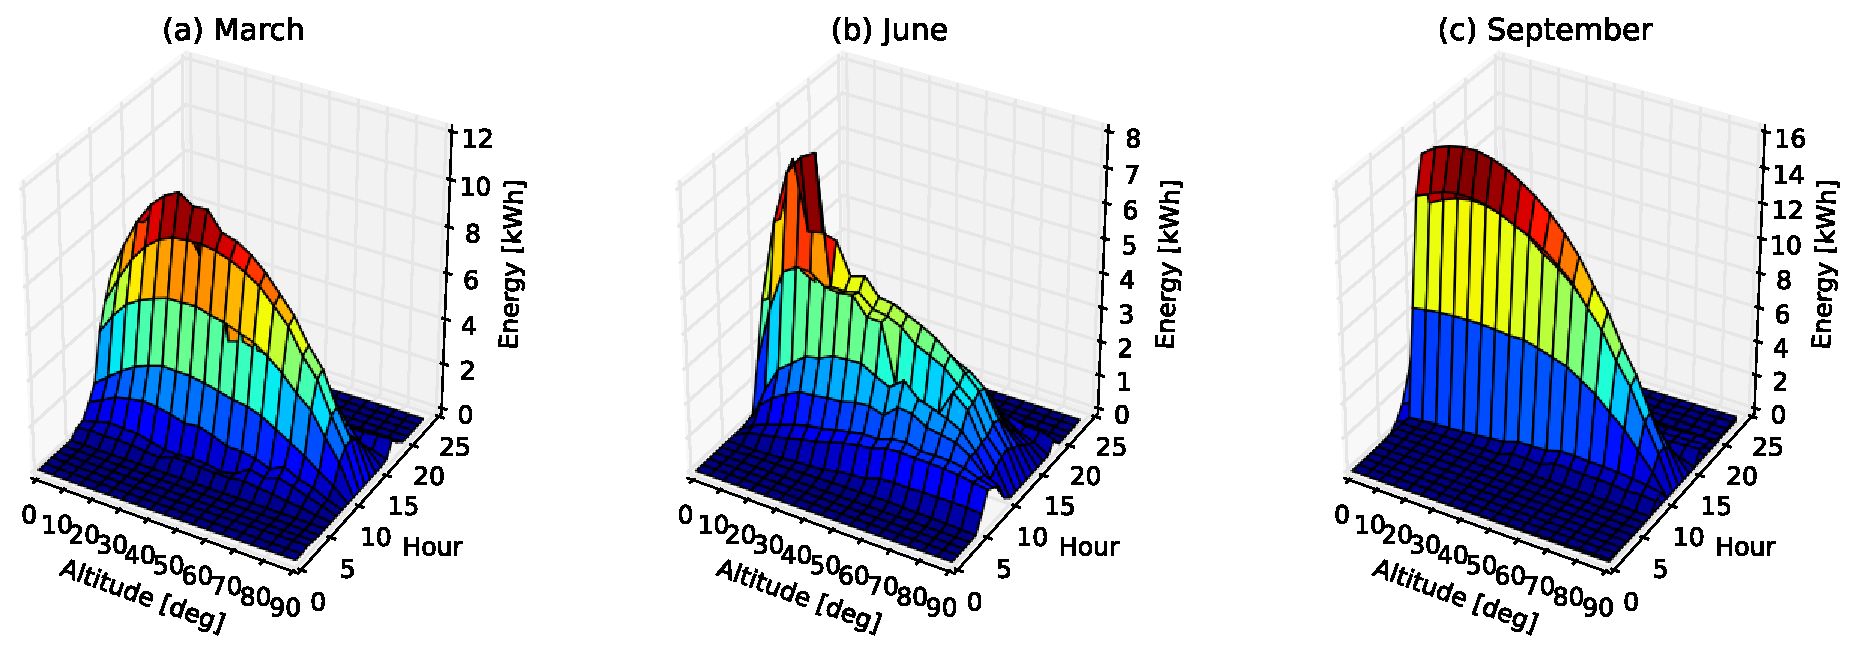
\includegraphics[width=1\textwidth, trim= 0cm 0cm 0cm 0cm,clip]{3d2}
		\caption{Energy benefits of the altitude actuation for the months of March (a), June (b) and September (c). Each plot displays one cumulative day in hourly resolution. The x-axis  represents the altitude angles, the y-axis corresponds to the hour of the day, and the z-axis represents the energy benefit of the actuation, i.e. the difference in energy usage between the evaluated angle and the angle that yields the worst overall energy usage for each hour.}
		\label{fig:3d}
		\end{center}
	\end{figure*}

	This overall behaviour corresponds well to the previously described results, that are depicted in Figure \ref{fig:monthly_altitude}, and shows why the angles that yield the optimum total energy, generally match the angles that optimise cooling and PV electricity production. A further interesting observation that can be made from this figure is the discontinuous curves for midday hours in summer. At an altitude angle of around $30^{\circ}$, the energy benefit reduces over-proportionally. This is caused by the PV electricity production, larger angles will increase longitudinal shading and therefore over proportionally reduce the energy yield. 


%\section{Radiation and PV Analysis}

	
	%To evaluate the performance of the radiation simulation, a grid-convergence study was performed and the optimum grid size for further simulations was found. The radiation results could then be used to calculate the PV electricity production, enabling the finding of optimum angles to maximise PV electricity production. The corresponding energy output was finally compared to a control strategy using solar tracking.

	%\subsection{Grid Convergence}

		%With a larger grid-size, results are less accurate. In order to study this effect, a grid convergence study was conducted. Figure \ref{f:gridConvergence} shows the grid size dependency of the total radiation on the asf. The colors in the first two plots on the upper left represent the hours of the day. One can see in the second plot - where the radiation is normalized by a division with the radiation for a grid-size of 12.5\,mm - that the results are significantly more accurate for morning and evening hours. This is caused by increased self-shading at midday hours. The colours in the third plot on the left show the dependency on different combinations. No clear pattern could be found here. Finally the average deviation is depicted in the fourth plot on the left and a box-plot with all deviations is shown on the right. It can be seen that a smaller grid-size leads to larger deviations. While for a grid-size of 400\,mm the average deviation is over 10\%, the deviation goes down to below 1\% for a grid size of 25\,mm. 25\,mm was therefore taken as the grid-size of all simulations, as it gives accurate results, while still being computationally feasible. 

		%\begin{figure*}
		%	\begin{center}
		%	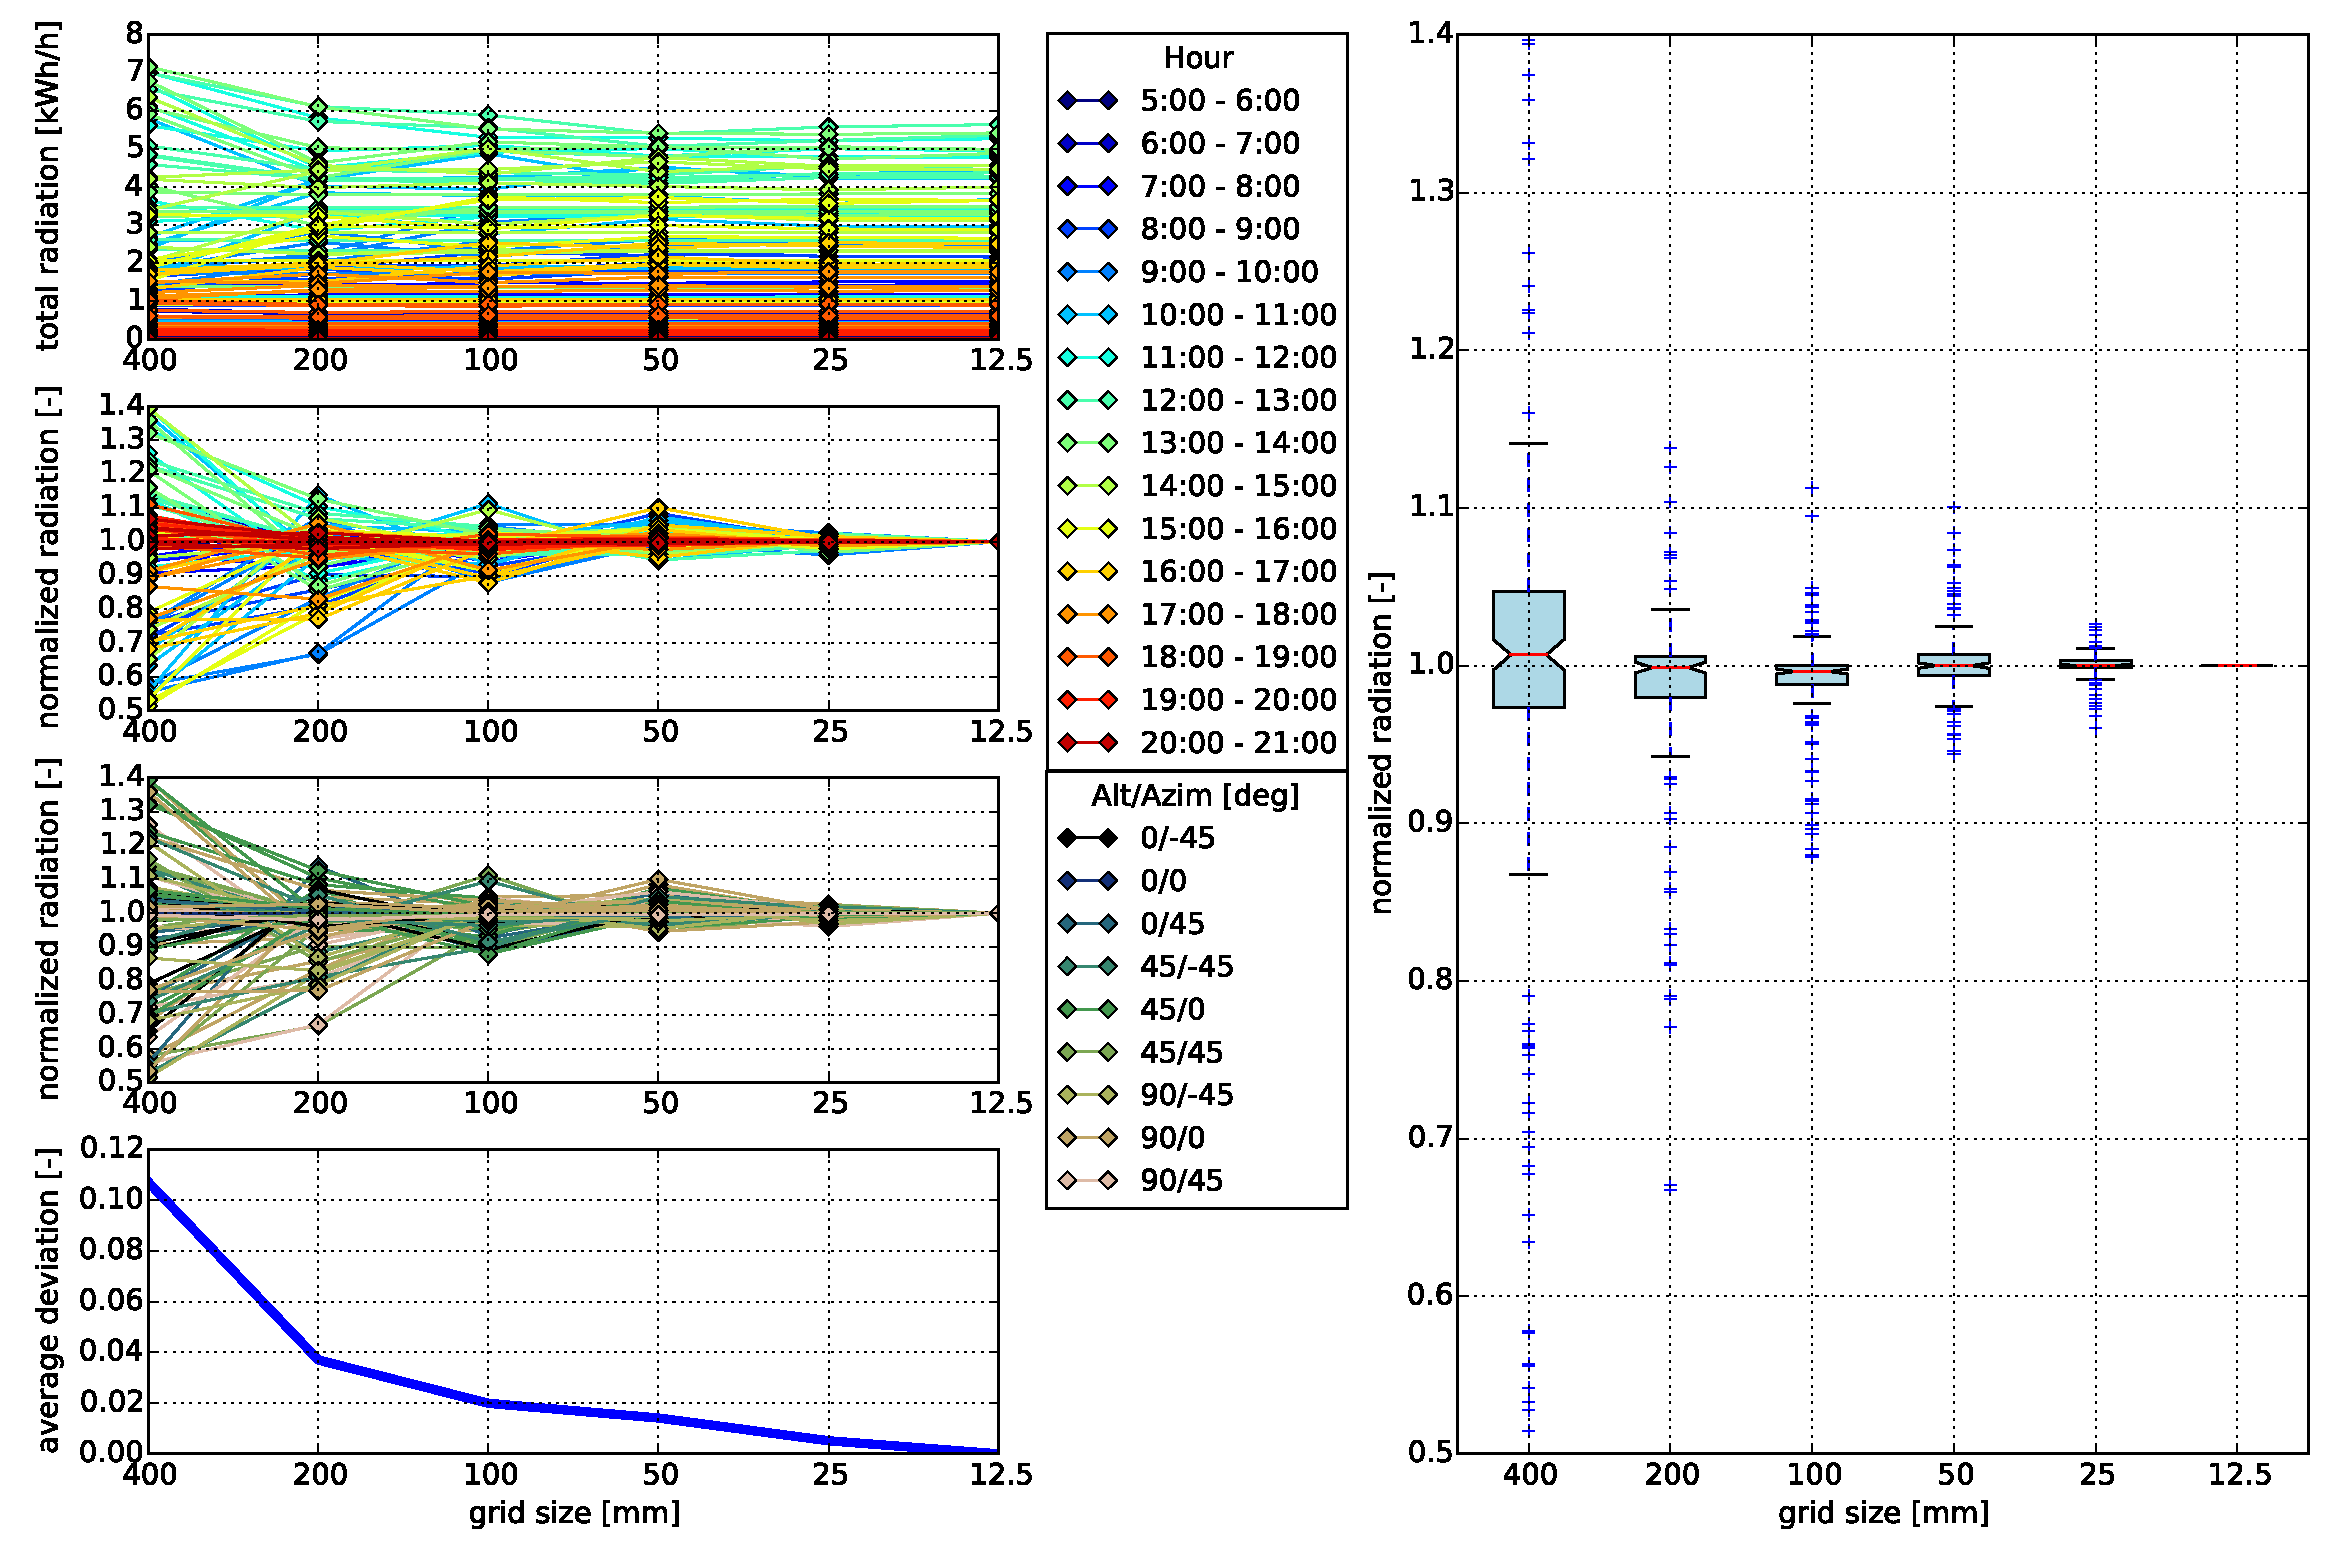
\includegraphics[width=\textwidth, trim= 0cm 0cm 0cm 0cm,clip]{gridConvergence.pdf}
		%	\caption{Grid convergence evaluation}
		%	\label{f:gridConvergence}
		%	\end{center}
		%\end{figure*}

	%\subsection{Comparison of Sun Tracking to Optimised Solution}
	%\label{ss:compareSunTracking}
\section{Comparison of Sun Tracking to Optimised Solution}
\label{s:compareSunTracking}

	As described in Section \ref{s:baseCase}, the optimisation of the PV electricity production were different from angles that would correspond to sun-tracking. To evaluate this difference, simulations using sun-tracking were compared to the optimising simulations, that are evaluating 49 different combinations (i.e. 7 different azimuth and altitude angles). 

	Figure \ref{f:compareSuntracking}a shows the radiation on the panels and compares it to the radiation that would be incident if there were no self-shading. It can be seen that while the radiation with sun-tracking is similar to the optimised solution, there are large losses in summer due to the self-shading. The total radiation on the panels is lower in summer than in spring and autumn. This can be explained by the higher altitude of the sun during summer months. The higher sun position results in increasing self-shading. 

	Figure \ref{f:compareSuntracking}b shows the PV electricity production for the two different control strategies, whereas the corresponding efficiencies are compared in Figure \ref{f:compareSuntracking}c. The PV electricity production - as well as the corresponding efficiency - of the optimised solution is significantly higher than the sun-tracking solution in the afternoon hours. This is caused by the layout of the PV panels, longitudinal shading causes high power losses \cite{hofer2016}, thus the optimised solution decreases the longitudinal shading compared to sun-tracking. Therefore, an optimising solution should be preferred over a sun-tracking approach for control strategy considerations. Finally, the temperature dependency of the PV electricity model can be observed from the graph that is detailing the efficiency, even though the radiation in the winter months is significantly lower than during the rest of the year, the corresponding efficiency is comparatively high because of the lower temperatures in the winter months. 

	\begin{figure*}
		\begin{center}
		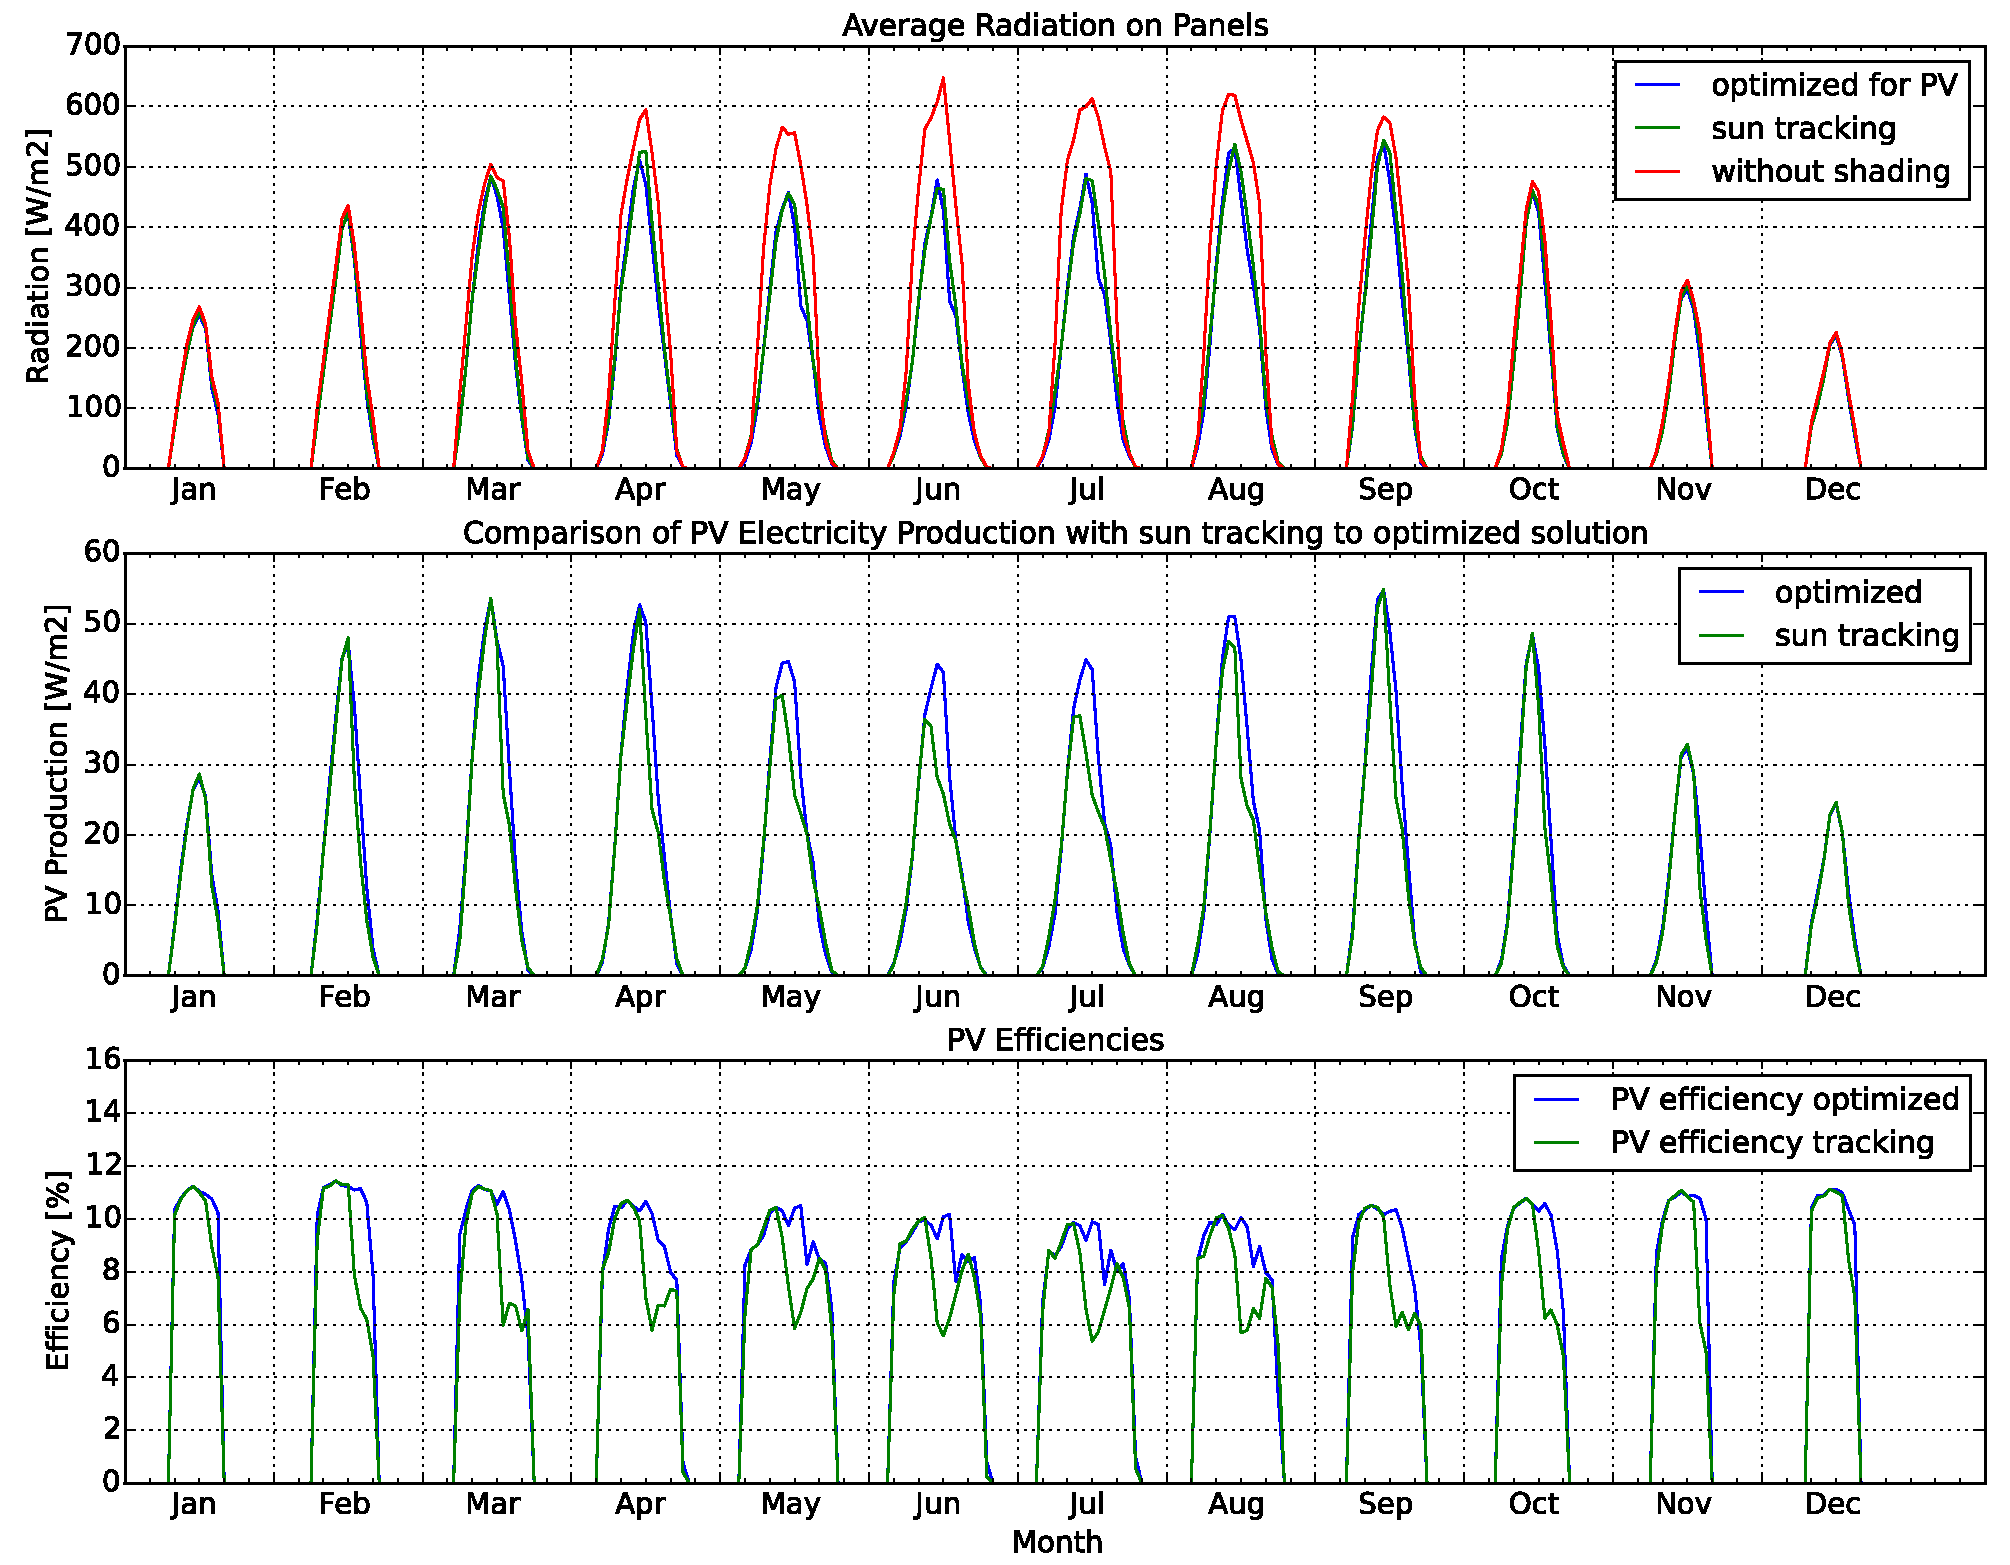
\includegraphics[width=\textwidth, trim= 0cm 0cm 0cm 0cm,clip]{PV}
		\caption{Comparison of optimised solution to sun-tracking. (a) Average radiation on panels compared to radiation without shading. While the radiation for sun-tracking is very similar to the radiation with the optimised angles, there are large losses caused by self-shading on the panels. (b) PV electricity production comparison. The optimised solution yields a significantly larger power output. (c) PV efficiency comparison. The optimised solution is able to stay at higher efficiencies than the sun-tracking approach.}
		\label{f:compareSuntracking}
		\end{center}
	\end{figure*}



\section{Sensitivity on Control Strategy Approach}
\label{s:tradeoffs}

	To evaluate further possibilities and limitations of the control strategy of the ASF, the tradeoffs between different strategies were visualised. Figure \ref{fig:tradeoffs}a shows the total energy demand used for heating, cooling, and lighting, the PV electricity production, as well as the total building demand and the net energy demand (building demand minus PV electricity production) for various control strategies. In Figure \ref{fig:tradeoffs}b the corresponding differences in energy of every control strategy to the individually optimised solution is shown. Even though the individual optimisation is not physically feasible, it is included in the evaluation because it serves as a good reference case, and tradeoffs between the different optimisation strategies can nicely be visualized. As expected, the overall optimisation has the smallest deviations from the individually optimised results. When comparing the different control strategies, one can see that especially cooling and PV need to be optimised, while the heating and lighting demand have a lower sensitivity on the control strategy. Another observation that can be gained is that the optimisation for cooling is not very beneficial for the PV electricity production. This corresponds to the results in the previous Section (\ref{s:compareSunTracking}) and is caused by the longitudinal shading, which the cooling optimisation does not take into account. However, the optimisation for PV electricity production has a smaller negative influence on the cooling demand. 

	\begin{figure*}[b!]
		\begin{center}
		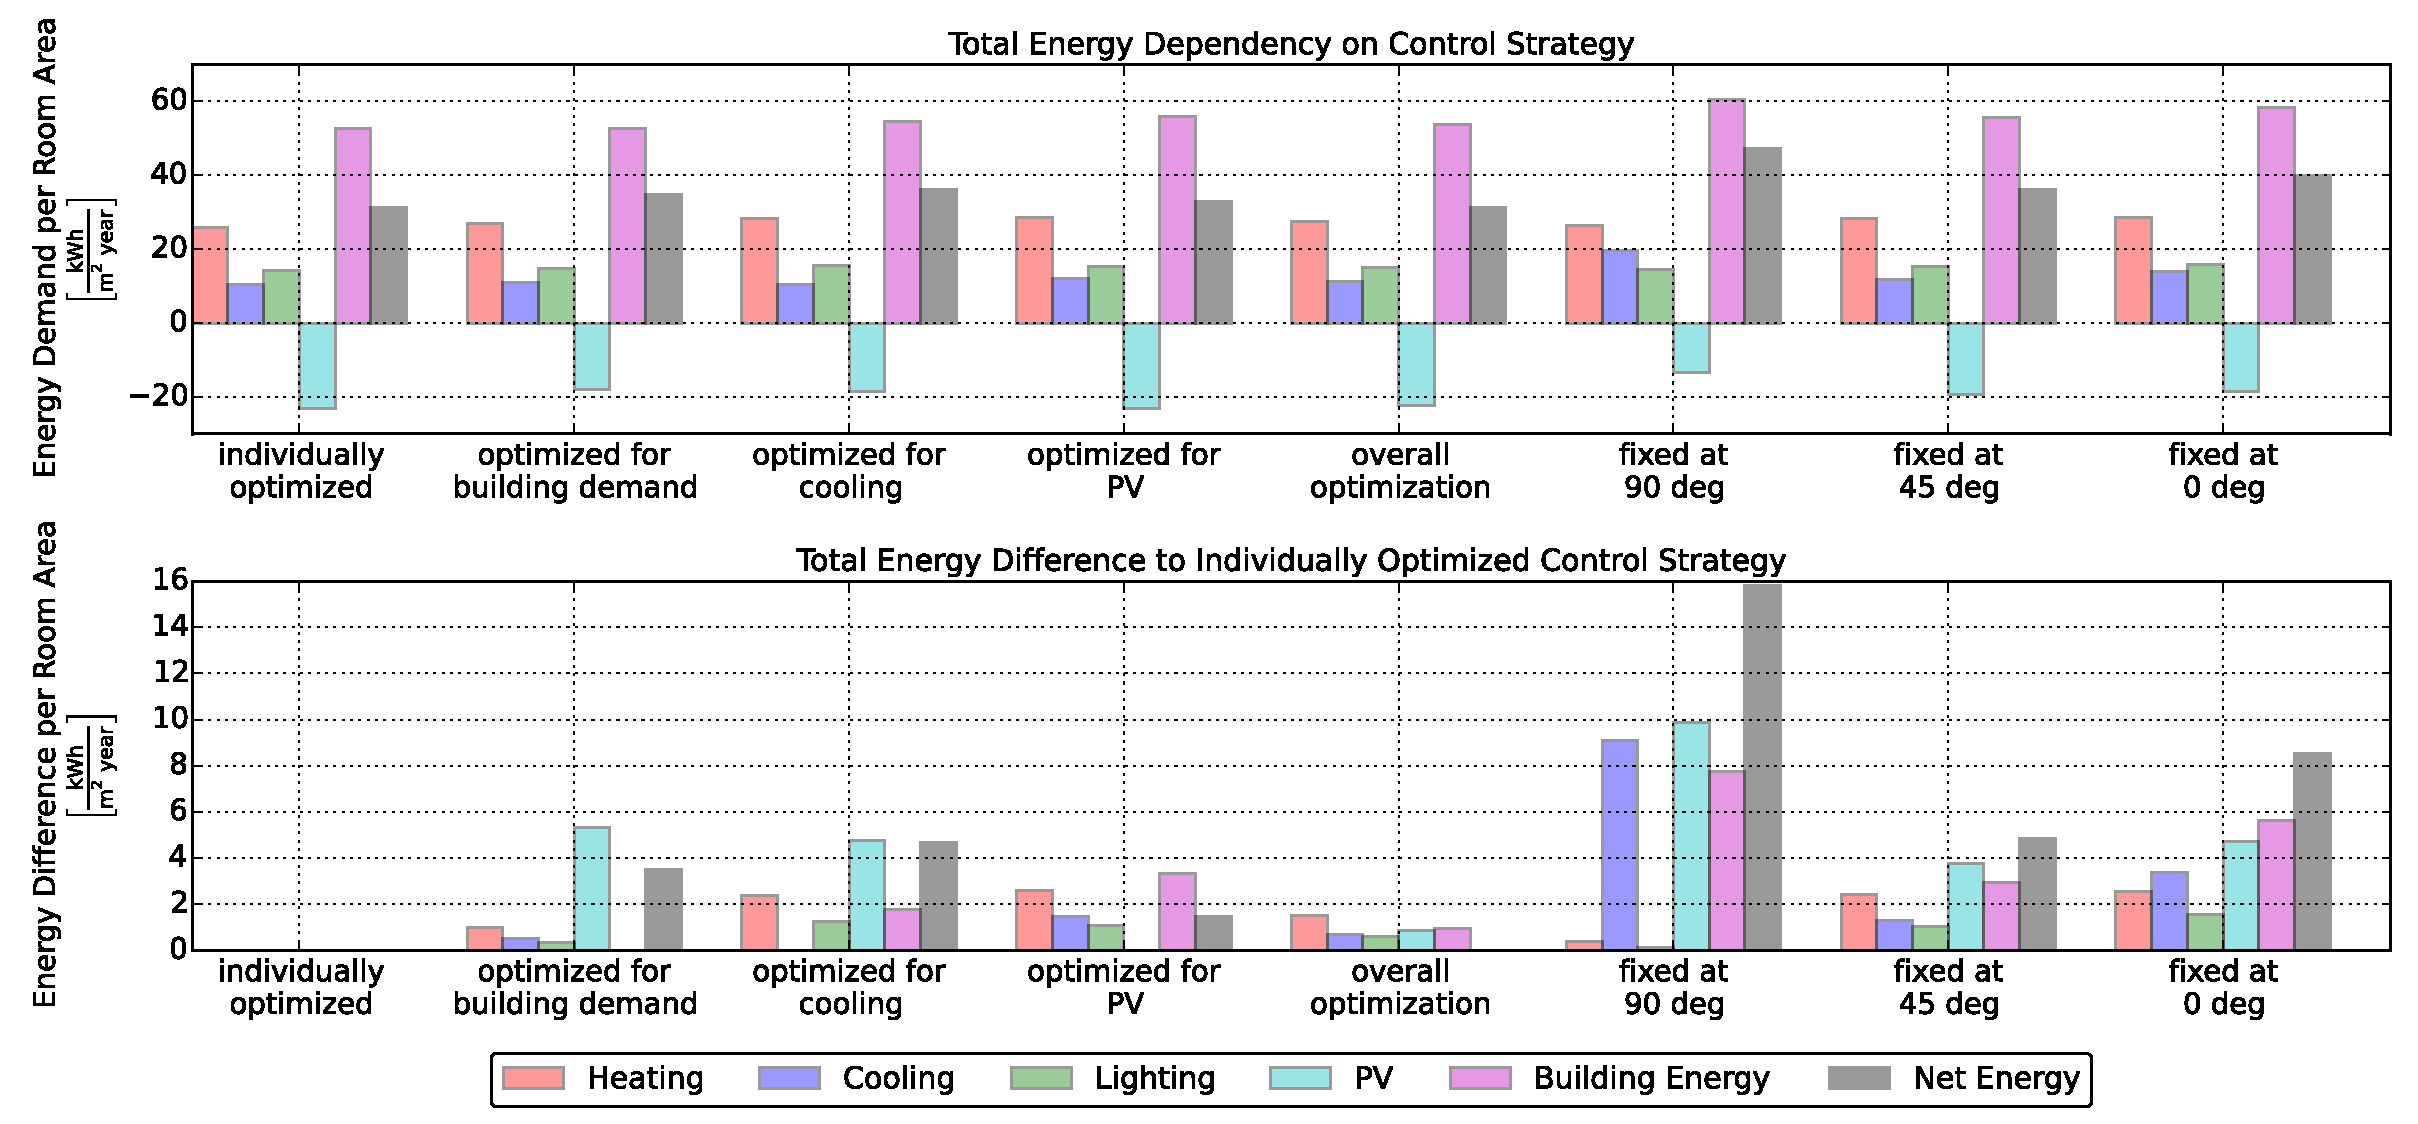
\includegraphics[width=1\textwidth, trim= 0cm 0cm 0cm 0cm,clip]{Tradeoffs}
		\caption{Comparison of different control strategies. (a) Total energy demand per room area. (b) Energy difference to individually optimised solution. While the individually optimised solution is not physically feasible, it is well suited for comparison and to emphasize the tradeoffs between the different optimisations.}
		\label{fig:tradeoffs}
		\end{center}
	\end{figure*}
	%\newpage

	This graph is part of the parametric simulation model, and can easily be adjusted to evaluate different building system parameters, as well as time periods. Further figures that visualise the same behaviour can be found in Appendix \ref{a:tradeoffs}.





\section{Orientation Analysis}

	%Evaluations of the facade for different building orientations were done with the base case of 5 azimuth and 5 altitude angles, corresponding to a total of 25 different combinations. This case was chosen in order to increase computational speed, simulations take less than half of the time that the 49 combination optimisation takes. Figure \ref{fig:buildingOrientation} shows the performance of the building and the facade for west, south-west, south, south-east and east orientations. (a) details the total energy demand for the optimised solution, (b) compares the performance of the optimised solution to a fixed solar facade at a $45\degree$ altitude angle, and (c) compares the performance of the optimised simulation to a simulation without external shading. Non surprisingly, the south facing facade produces the most electricity. It also has the lowest building energy consumption, mainly because of a low energy demand for heating and cooling. It was found that the PV apertures should be oriented parallel to the upper left edge for facades that are west or south-west oriented, whereas they should be oriented parallel to the upper right edge for east or south-east oriented facades. This is caused by the shading patterns, longitudinal shading needs to be prevented as described in Section \ref{s:compareSunTracking}. Furthermore, it can be observed that an east facing building uses less heating than a west facing building, which could be explained with the previous observation that heating is most important during morning hours. For similar reasoning the east facing building needs more cooling energy than the west facing building, because the room heats up in the morning and will not naturally cool down before outdoor temperatures drop in the evening. Interestingly, PV production is higher for the west facing facade than for the east facing facade. The cause for this is probably because of conflicts in optimising cooling and PV electricity production at the same time, as cooling is more dominant for the east facing building. Overall, the south-east facing facade performs the best, when compared to the corresponding reference cases. It can clearly be seen, that this performance increase mainly comes from the high cooling demand, the benefits of the facade for the cooling energy use outweigh the lower benefit of the PV electricity supply. 
	Evaluations of the facade for different building orientations were done with the base case of 5 azimuth and 5 altitude angles, corresponding to a total of 25 different combinations. This case was chosen in order to increase computational speed. In comparison to the optimisations with 49 combinations, simulations take less than half the time.%Simulations take less than half of the time that the 49 combination optimisation takes. 

	Figure \ref{fig:buildingOrientation} shows the performance of the building and the facade for west, south-west, south, south-east and east orientations. (a) details the total energy demand for the optimised solution, as expected, the south facing facade produces the most electricity. It also has the lowest building energy consumption, mainly because of a low energy demand for heating and cooling. It was found that the PV apertures should be oriented parallel to the upper left edge for facades that are west or south-west oriented, whereas they should be oriented parallel to the upper right edge for east or south-east oriented facades. This is caused by the shading patterns. Longitudinal shading needs to be prevented as described in Section \ref{s:compareSunTracking}. Furthermore, it can be observed that an east facing building uses less heating than a west facing building, which could be explained by the previous observation that heating is most important during morning hours. For similar reasoning, the east facing building needs more cooling energy than the west facing building because the room heats up in the morning and will not naturally cool down before the outdoor temperatures decrease in the evening. Interestingly, PV production is higher for the west facing facade than for the east facing facade. The cause for this is probably because of conflicts in optimising cooling and PV electricity production at the same time, as cooling is more dominant for the east facing building. 

	As for the ASF performance, the south-east facing facade yields the highest energy benefits. This becomes apparent when comparing the energy savings of the ASF to a fixed facade at a $45\degree$ altitude angle, or to a building with no external shading, as described in Figure \ref{fig:buildingOrientation} (b) and (c), respectively. It can clearly be seen, that this performance increase mainly comes from the high cooling demand. The benefits of the facade for the cooling energy use outweigh the lower benefit of the PV electricity supply. 

	\begin{figure*}
		\begin{center}
		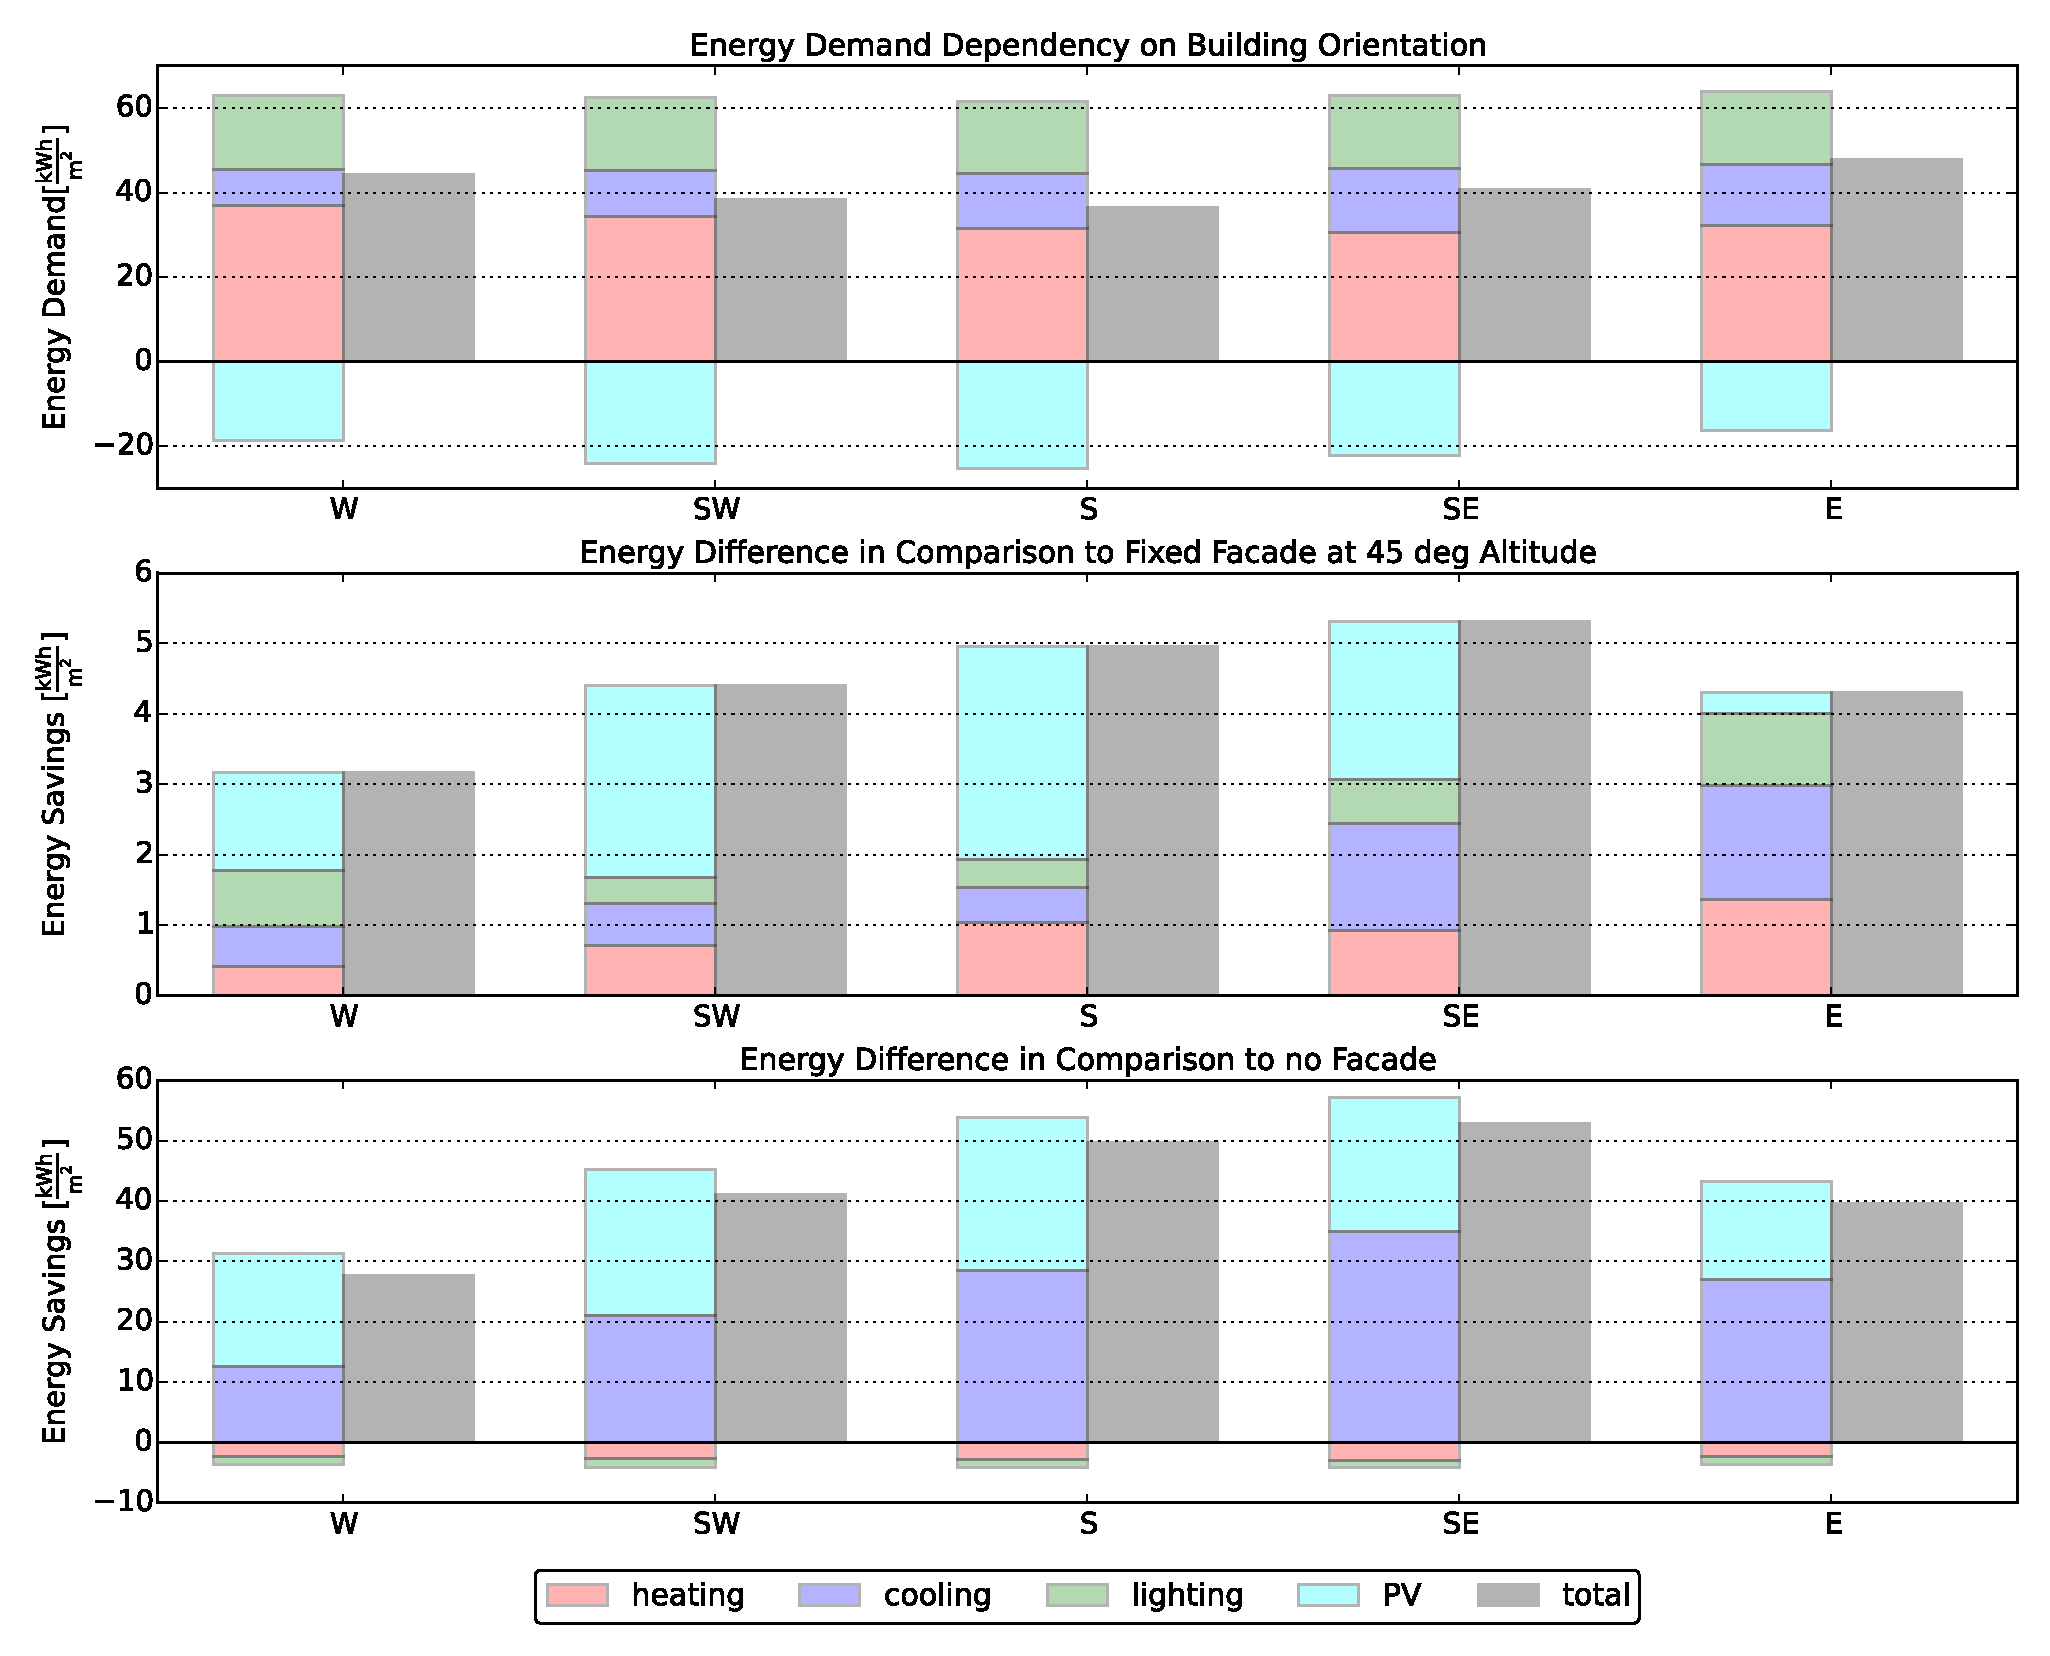
\includegraphics[width=1\textwidth, trim= 0cm 0.7cm 0cm 2.5cm,clip]{orientation}
		\caption{Energy demand in dependence of building orientation. (a) Total Energy Demand per room area, a south facing room has the lowest building energy demand while simultaneously maximising the PV-electricity production. (b) Energy Savings per room area of optimised solution compared to a fixed solar facade at $45\degree$ altitude. (c) Energy Savings per room area of optimised solution compared to a building without external shading. The energy benefit of the south-east facing ASF is the highest, mainly due to a better cooling performance.}
		\label{fig:buildingOrientation}
		\end{center}
	\end{figure*}

	%\newpage

\section{Location Analysis}

	%Similarly to the orientation analysis, the location of the building was evaluated. In Figure \ref{fig:buildingLocation}, the corresponding energy performance of an ASF is shown for the locations Helsinki, Zurich, Madrid, and Cairo. (a) shows the net energy demand for the different locations, (b) details the energy savings compared to a fixed solar facade at a $45\degree$ altitude angle and (c) compares the net energy demand of a building with an ASF to a building without external shading. As for the building energy demand, it can clearly be seen that the further south a building is, the higher the cooling load and the lower the heating demand. The lighting however is similar in all cases. Interestingly, the PV electricity output is highest in Madrid. This can be explained by the altitude of the sun, in Cairo the average altitude is higher and therefore also the self-shading on the panels. As Madrid also shows the lowest net building energy demand, it can be said that the system is most efficient for this location. An analysis of the energy savings visualizes the impact of the location on the performance of the ASF even better. It can clearly be seen, that the warm and sunny locations of Madrid and Cairo have significantly larger energy savings than the ones in Helsinki and Zurich. This is caused by the large benefits of the ASF on reducing cooling as well as increasing the PV electricity output. 
	Similarly to the orientation analysis, the location of the building was evaluated. In Figure \ref{fig:buildingLocation}, the corresponding energy performance of an ASF is shown for the locations Helsinki, Zurich, Madrid, and Cairo. (a) shows the net energy demand for the different locations, it can clearly be seen that the further south a building is, the higher the cooling load and the lower the heating demand. The lighting however is similar in all cases. Interestingly, the PV electricity output is highest in Madrid. This can be explained by the altitude of the sun, in Cairo the average altitude is higher and therefore also the self-shading on the panels. As Madrid also shows the lowest net building energy demand, it can be said that the system is most efficient for this location. An analysis of the energy savings visualizes the impact of the location on the performance of the ASF even better. Therefore, the energy savings compared to a fixed solar facade at a $45\degree$ altitude angle and to a building without external shading are shown in Figure \ref{fig:buildingLocation} (b) and (c), respectively. The warm and sunny locations of Madrid and Cairo have significantly larger energy savings than the ones in Helsinki and Zurich. This is caused by the large benefits of the ASF on reducing cooling as well as increasing the PV electricity output. 

	\begin{figure*}
		\begin{center}
		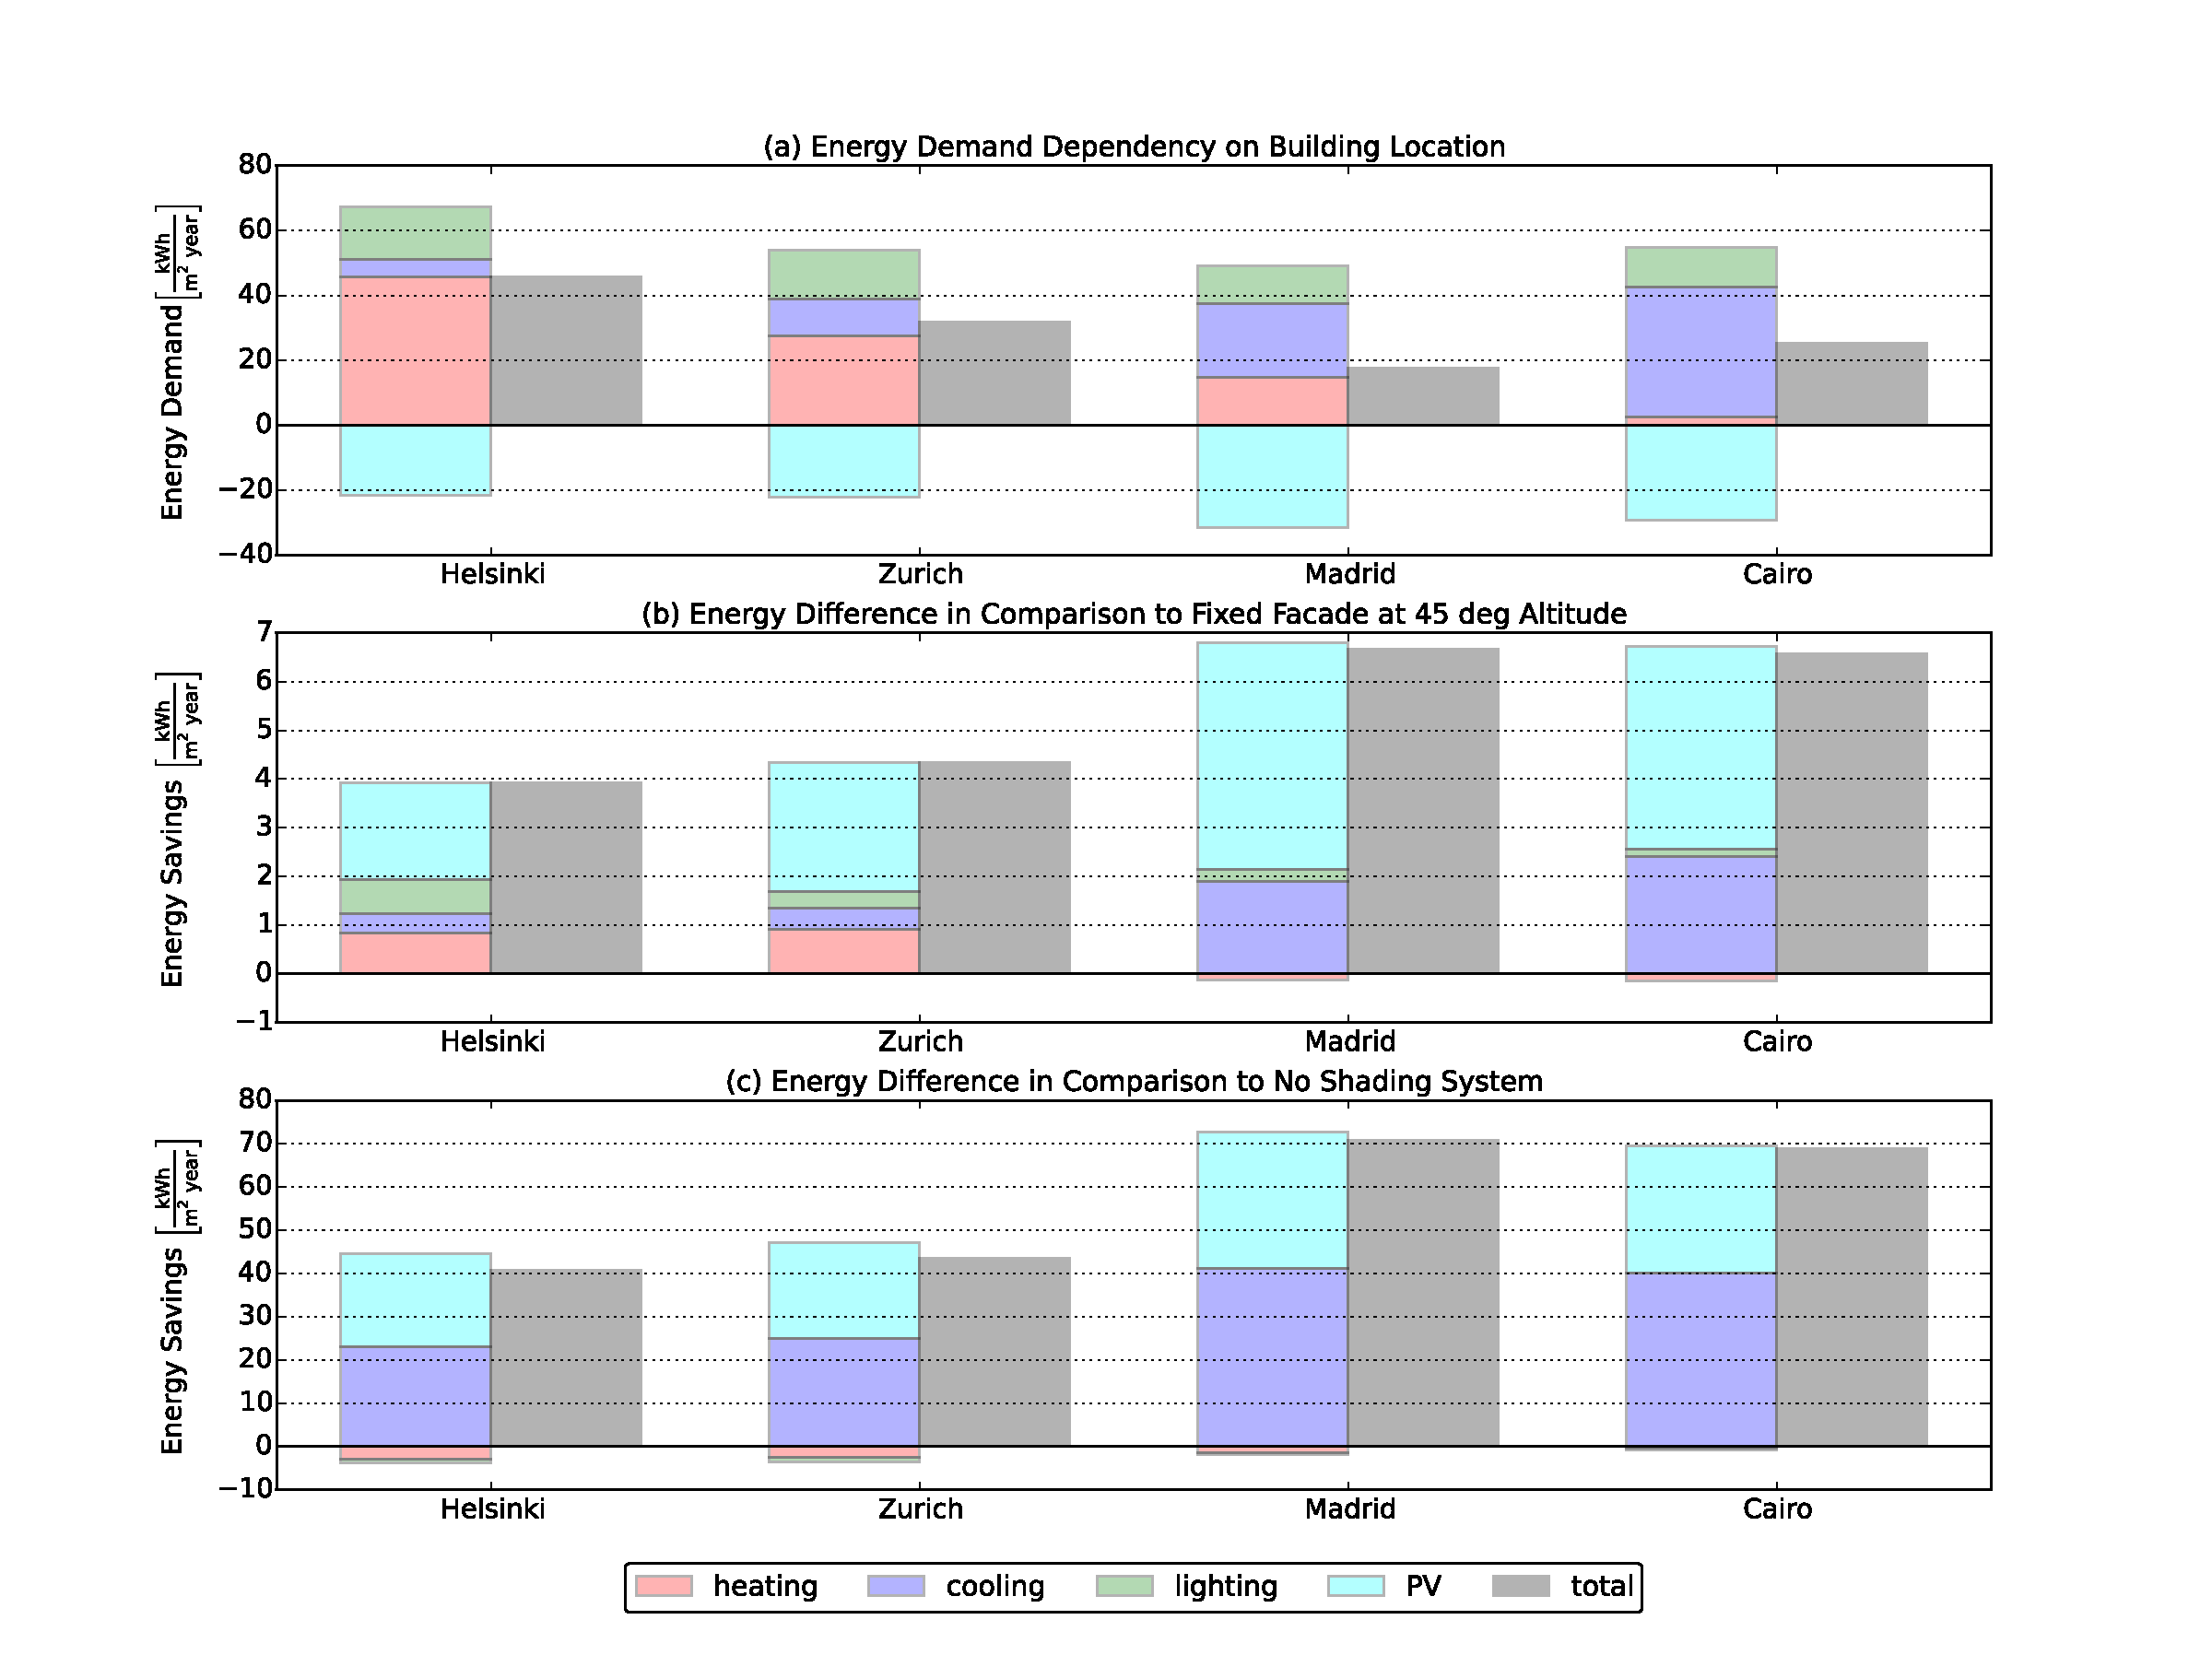
\includegraphics[width=1\textwidth, trim= 0cm 0.7cm 0cm 2.5cm,clip]{Location}
		\caption{Energy demand in dependence of building location. (a) Total Energy Demand per room area, Madrid yields the lowest building energy demand while simultaneously maximising the PV-electricity production. (b) Energy Savings per room area of optimised solution compared to a fixed solar facade at $45\degree$ altitude. (c) Energy Savings per room area of optimised solution compared to a building without external shading. The energy benefit of the ASF for the warm and sunny regions is much greater than for the colder regions, this is due to a higher significance of cooling and increased electricity production of the PV panels.}
		\label{fig:buildingLocation}
		\end{center}
	\end{figure*}
\section{Sensitivity on Building System Parameters}

	A sensitivity analysis was done for the heating coefficient of performance (COP), cooling COP, lighting load, and infiltration rate. The results are shown in Figure \ref{fig:sensitivity}. Figure \ref{fig:sensitivity}a shows the energy savings per square meter of room area compared to a fixed solar facade at an angle of $45\degree$, whereas Figure \ref{fig:sensitivity}b shows the energy savings compared to a building without any PV modules or shading devices. The highlighted bar in each subplot represents the base case of the simulation with the same settings, therefore it has the same height for each parameter evaluation in the same row and serves as a reference. It can be seen that while the heating and cooling COP have large influences on the energy savings, the influence of the lighting load and the infiltration rate are significantly smaller. Especially a low COP for heating and cooling have a strong impact on the performance. For cooling, it becomes clear that an ASF is especially beneficial with inefficient cooling. As for the heating, it depends on the comparison case. While the energy savings are larger for a small heating COP when comparing it to a fixed solar facade at a $45\degree$ angle, they are smaller when comparing it to a building without external shading. This can be explained with the importance of heating for each of the two reference cases. A building without any shading naturally has a lower heating demand than a building with shading. When the heating COP is very small, which means that the energy demand for the heating is larger, it is relatively more efficient to have a building without shading than with shading. However, an ASF is still beneficial, as even with the lowest evaluated heating COP of 1 - corresponding to electrical heating - there are still significant overall energy benefits. 

	\begin{figure*}
		\begin{center}
		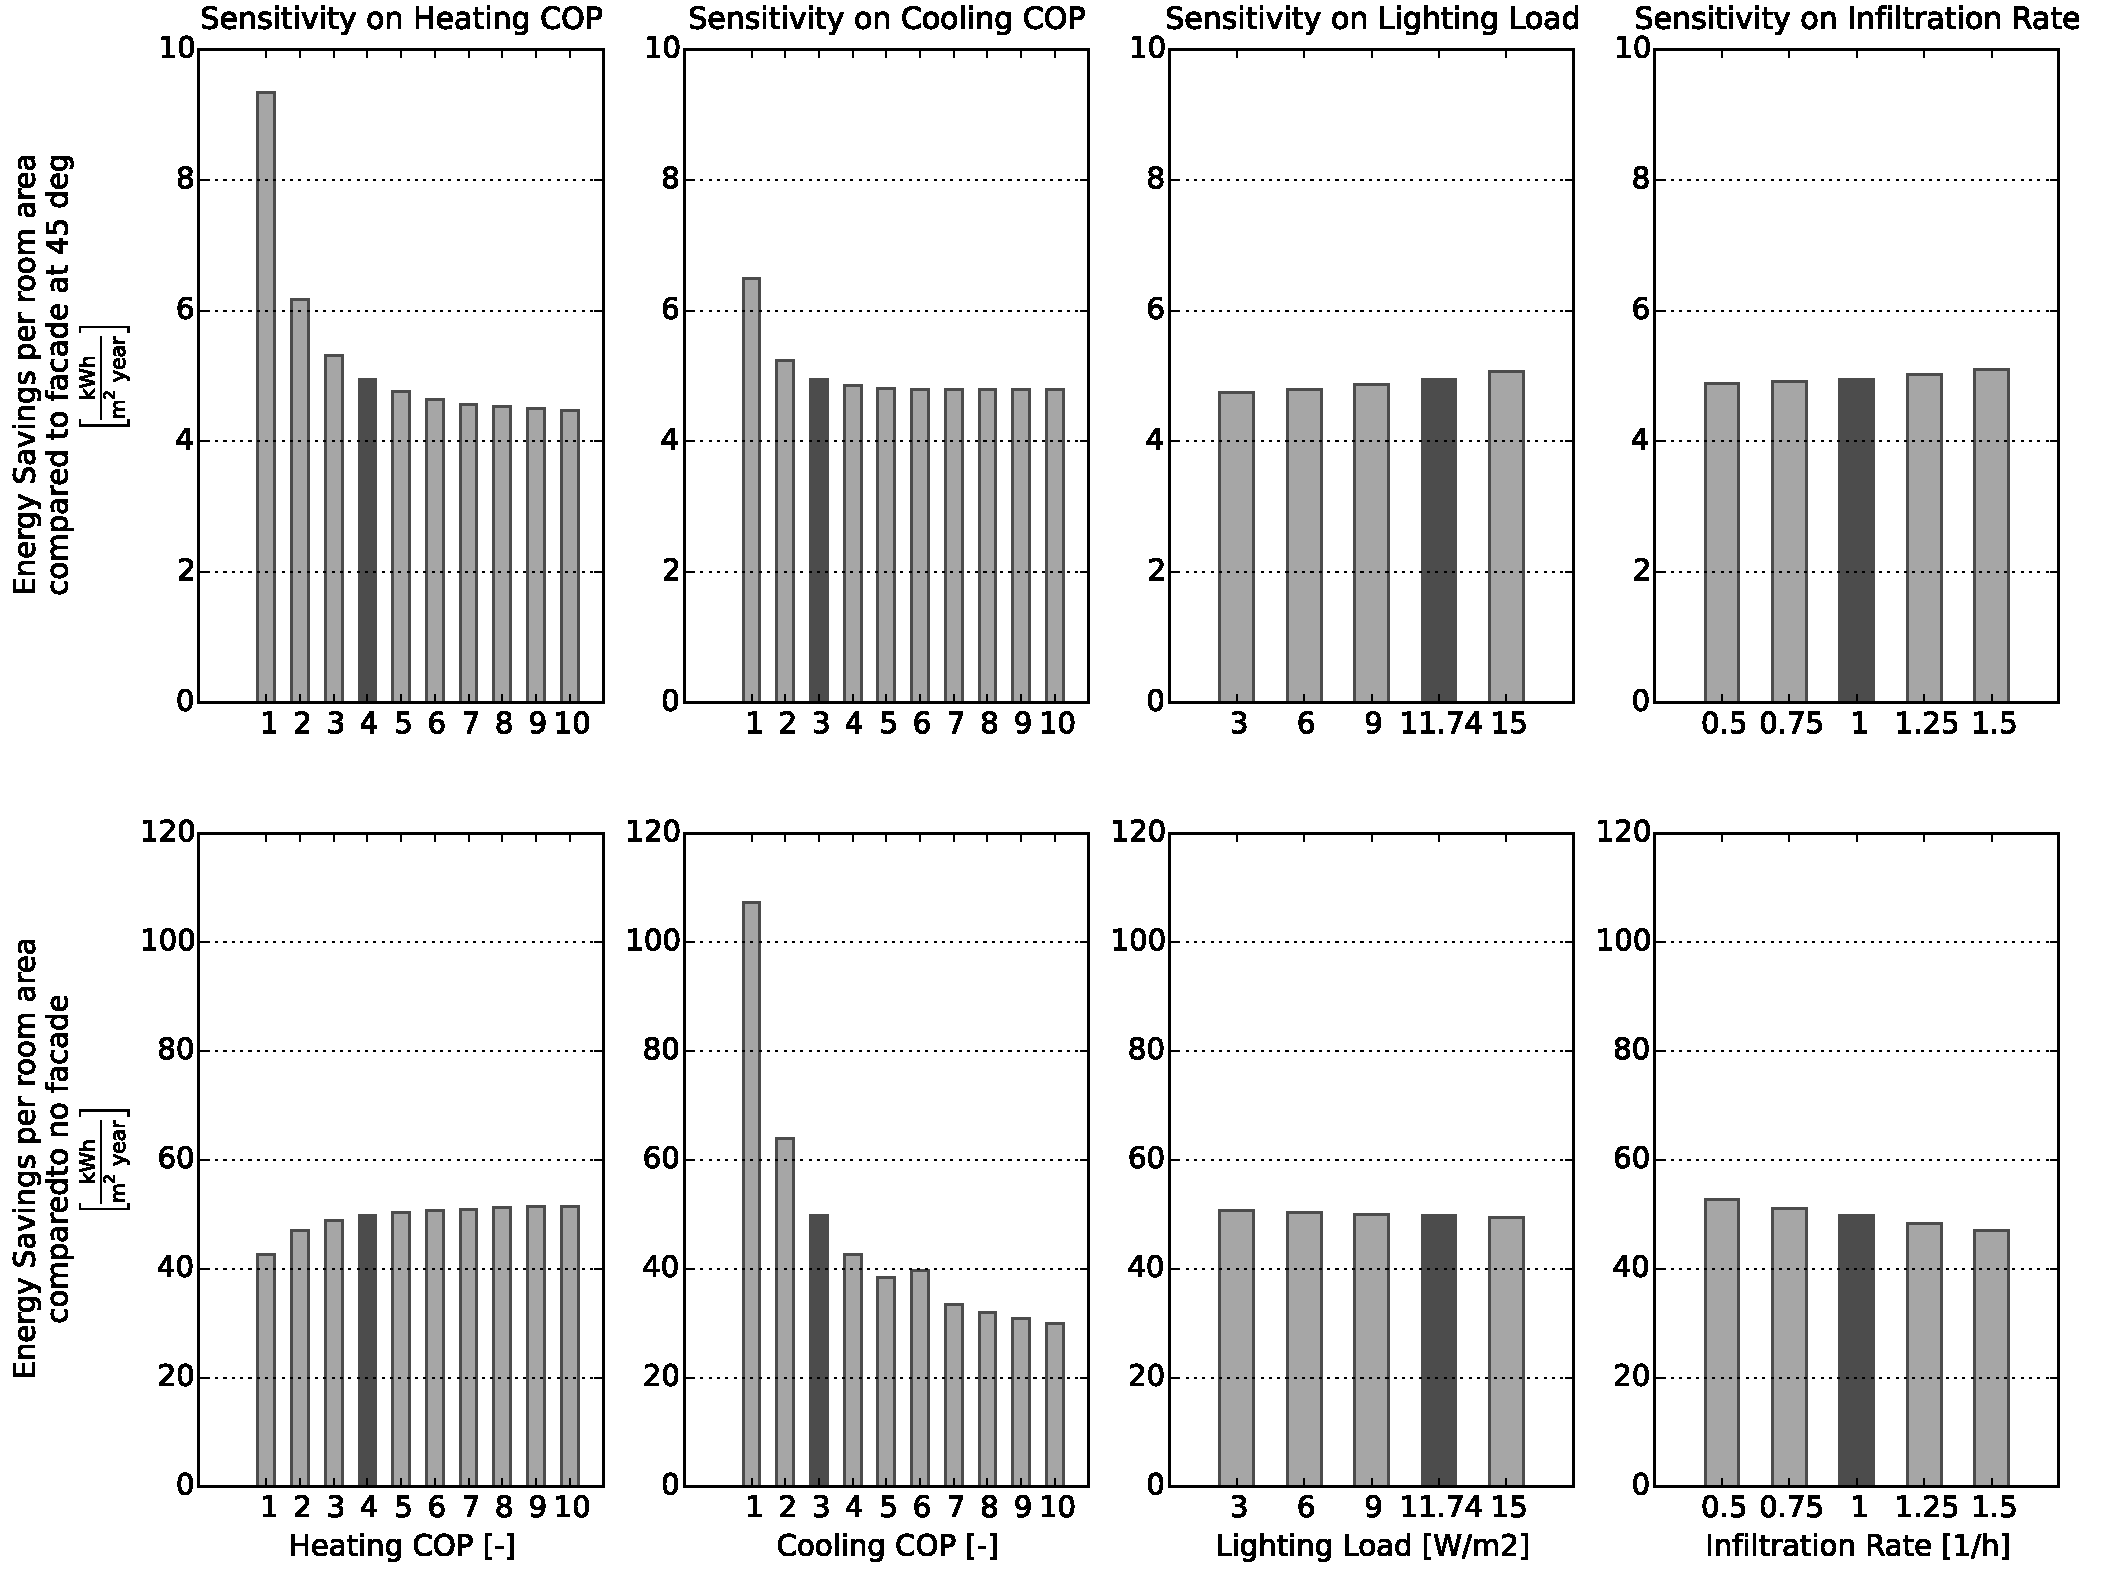
\includegraphics[width=\textwidth, trim= 0cm 0cm 0cm 0cm,clip]{buildingSensitivity}
		\caption{Sensitivity analysis of energy savings during one year. From left to right, sensitivities on heating COP, cooling COP, lighting load, and infiltration rate. The top row (a) shows the energy savings compared to a fixed solar facade at a $45\degree$ altitude angle, the bottom row (b) shows the energy savings compared to a room without shading or PV modules. The emphasized bar in every subplot corresponds to the basecase settings, all of them have the same height as they correspond to the same simulation. }
		\label{fig:sensitivity}
		\end{center}
	\end{figure*}

\section{Evaluation of Different Combination Settings}
	
	With the parametric model, it is possible to evaluate every thinkable set of angle combinations. However, computational limitations require a discrete set of angles. In order to assess the influence of the chosen angle combinations on the performance of the ASF, various different combinations have been evaluated. In Figure \ref{fig:combinations}, the energy savings of various simulation combinations are shown, compared to a fixed solar facade at a $45\degree$ altitude angle (a), as well as to a building without external shading (b). Variations include evaluations of using only one axis actuation (i.e. either a fixed azimuth or a fixed altitude angle), as well as using multiple angles for both altitude and azimuth actuation. The angles were always distributed equally between $0\degree$ and $90\degree$ or between $-45\degree$ and $45\degree$ for the altitude and azimuth variations, respectively. When using multiple angles, the maximum and minimum actuation angle was always included. For example, an analysis using three altitude and three azimuth angles used $0\degree$, $45\degree$ and $90\degree$ for the altitude variations, while the azimuth variations would include the angles $-45\degree$, $0\degree$ and $45\degree$. It can be seen that the more angles are used, the higher the energy savings become. However, with an increasing number of combinations comes a corresponding increasing amount of computation time. While an evaluation of five different combinations takes approximately four hours with the machine that was used, it goes up to 20 hours for the evaluation of 25 combinations or even 50 hours for the evaluation with 49 combinations. Higher energy savings will definitely be possible with the use of an increasing number of combinations, though the benefit of increasing the number of combinations will gradually go down to zero. 
	\begin{figure*}
		\begin{center}
		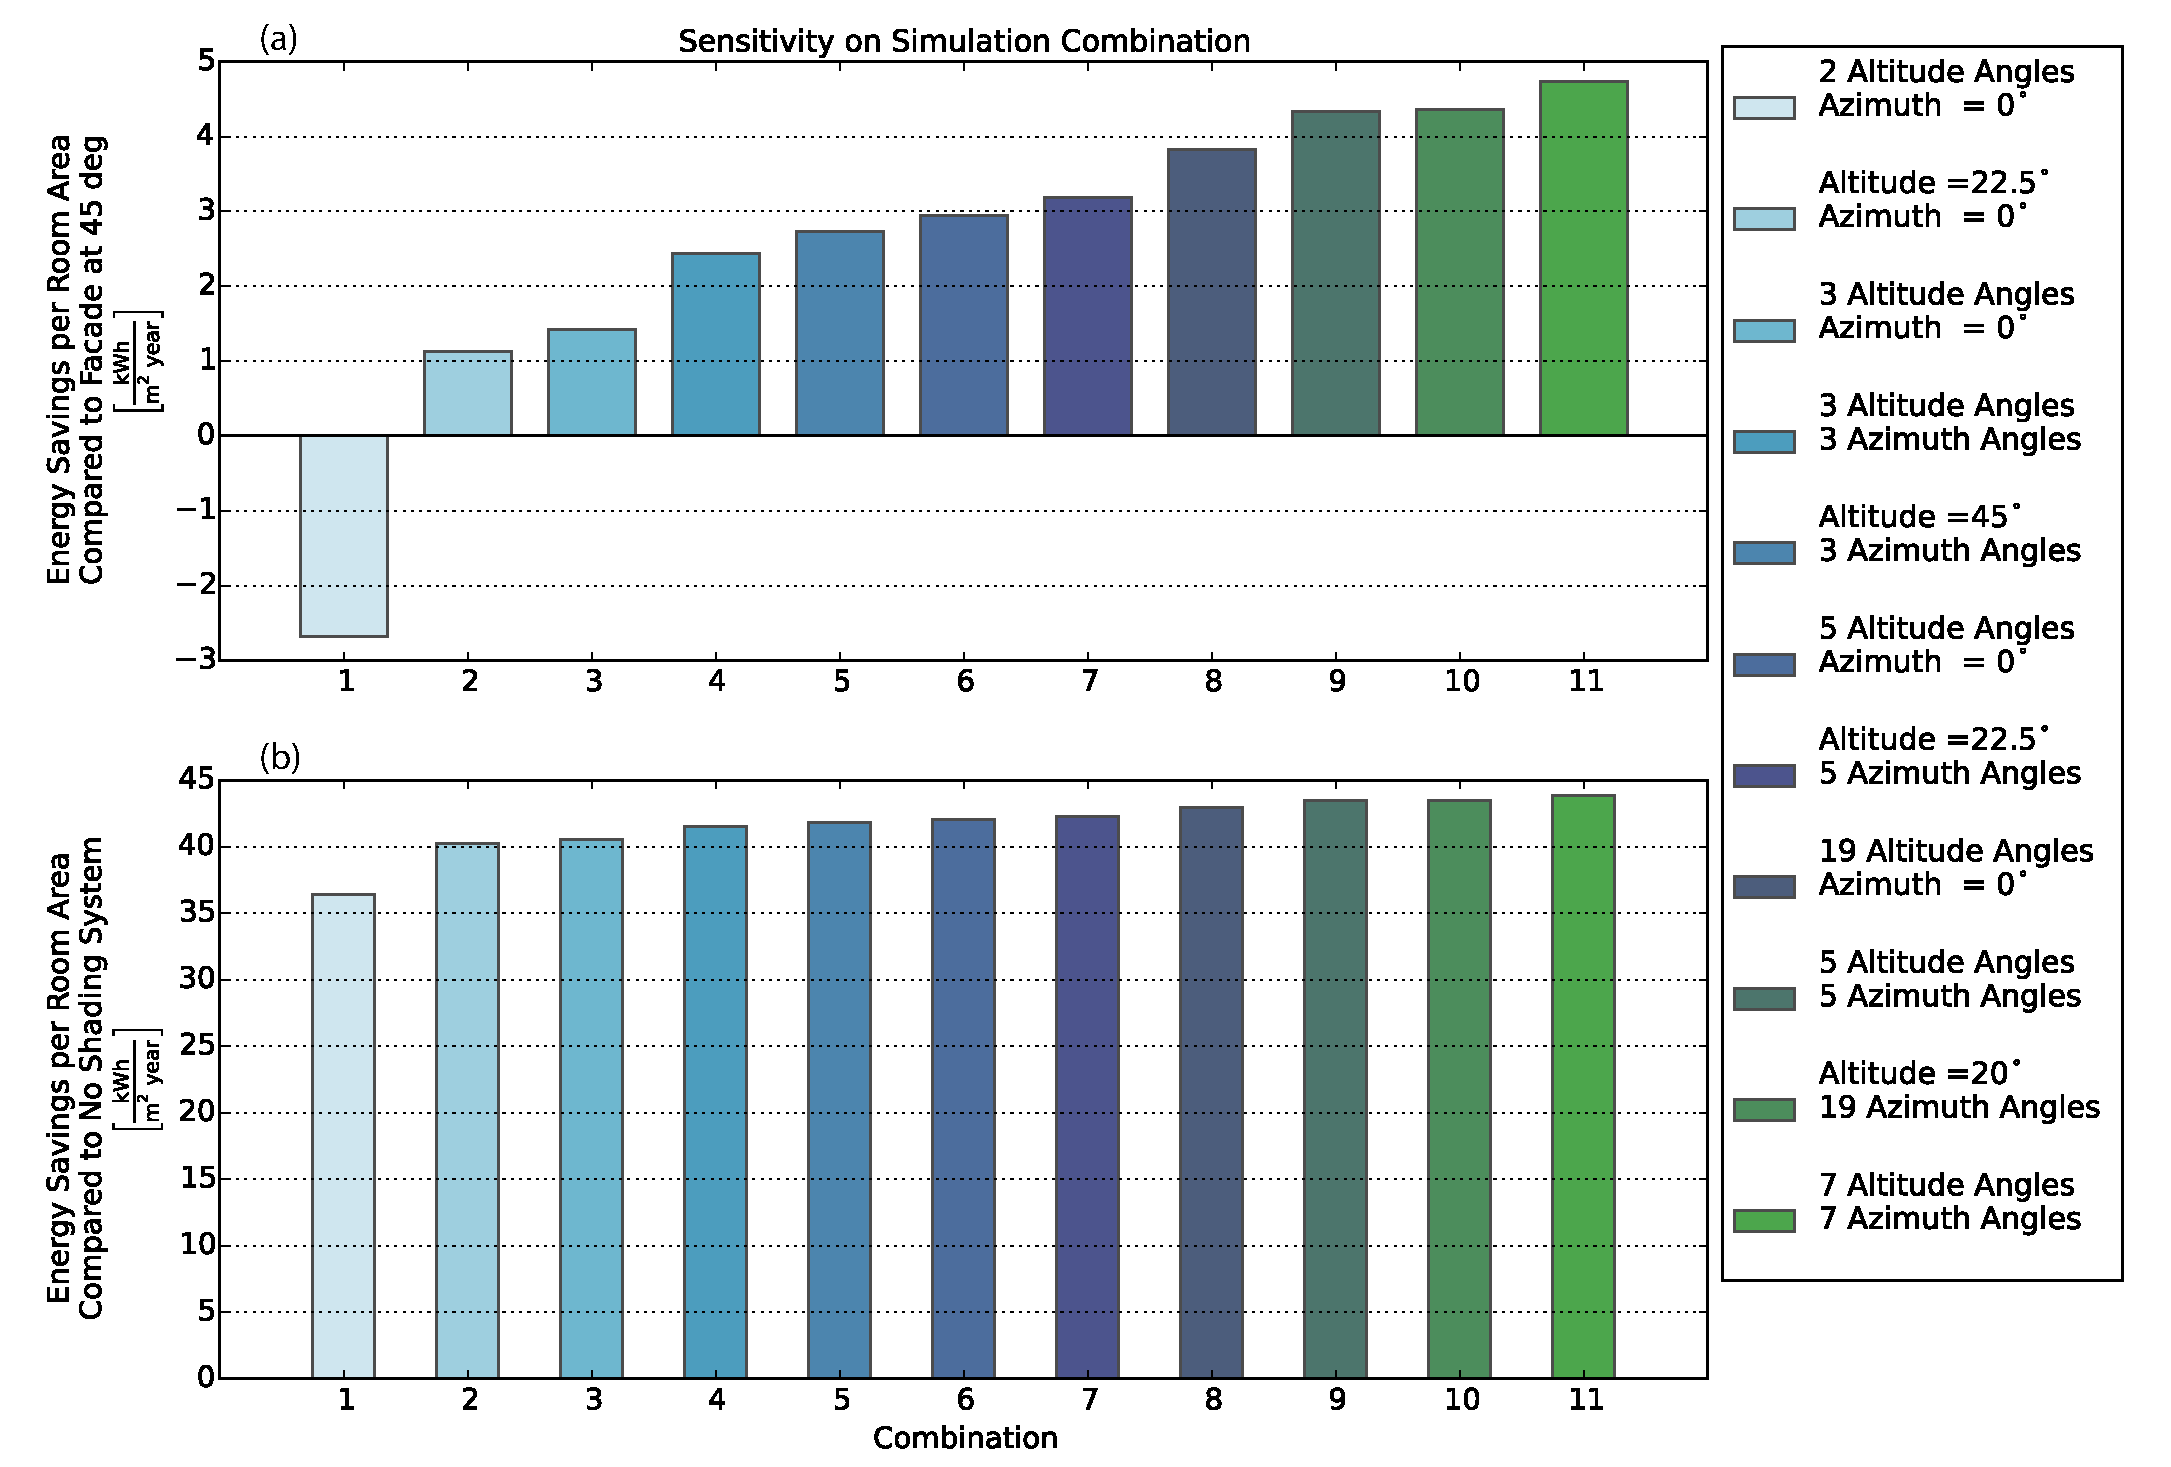
\includegraphics[width=1\textwidth, trim= 0cm 0cm 0cm 0cm,clip]{combinations2}
		\caption{Comparison of different combination settings. (a) shows the energy savings compared to a fixed facade at a $45\degree$ altitude, (b) shows the savings in comparison to a building with no external shading.}
		\label{fig:combinations}
		\end{center}
	\end{figure*}
	
\section{Potential of Independent Actuation}
	Independent actuation of the panels is one of the key advantages of the ASF that have to be closely evaluated. In order to quantize the potential of individual actuation, evaluations were performed by splitting the ASF into clusters. Due to computational limitations, especially on the radiation simulation, simplified geometries were used for the radiation evaluation. Ten panels in four rows with two clusters and eight panels in three rows with three clusters were used, rather than the 50 panels of the reference case with one cluster. Furthermore, only the months of March, June, September, and December were evaluated. The two cluster evaluation was done for the reference case with five azimuth and five altitude angles. The evaluation with three clusters was done only for altitude variations, with 5 angles in each cluster. A visualization of the cluster comparison is shown in Figure \ref{fig:cluster}. The left column details the comparison of two clusters against one cluster, whereas the right column shows the comparison of three clusters to one cluster. Figure \ref{fig:cluster}a shows the net power use of the building for an average day of June, (b) depicts the corresponding power difference, and (c) details the average energy saving for the months of March, June, September and December. When looking at the power difference, it can be seen that the main benefit of using multiple clusters comes from deviations around noon and in the afternoon. This can be explained with the self-shading on the panels, as the facade has to optimise the longitudinal shading mainly in the afternoon (as described in Section \ref{s:compareSunTracking}). Therefore, the losses due to conflicts between cooling and PV can be reduced with the use of independent actuation. The comparison of the energy savings shows the impact on the conflicting energy yields. In the two cluster case, the energy benefits from heating and PV electricity are reduced, while cooling and lighting become more beneficial. The corresponding total energy demand could be reduced by approximately 1\%. For three clusters, there are benefits for cooling, lighting and PV, though heating still brings some drawbacks. However, the corresponding total energy demand was reduced by 2.3\%.

	\begin{figure*}
		\begin{center}
		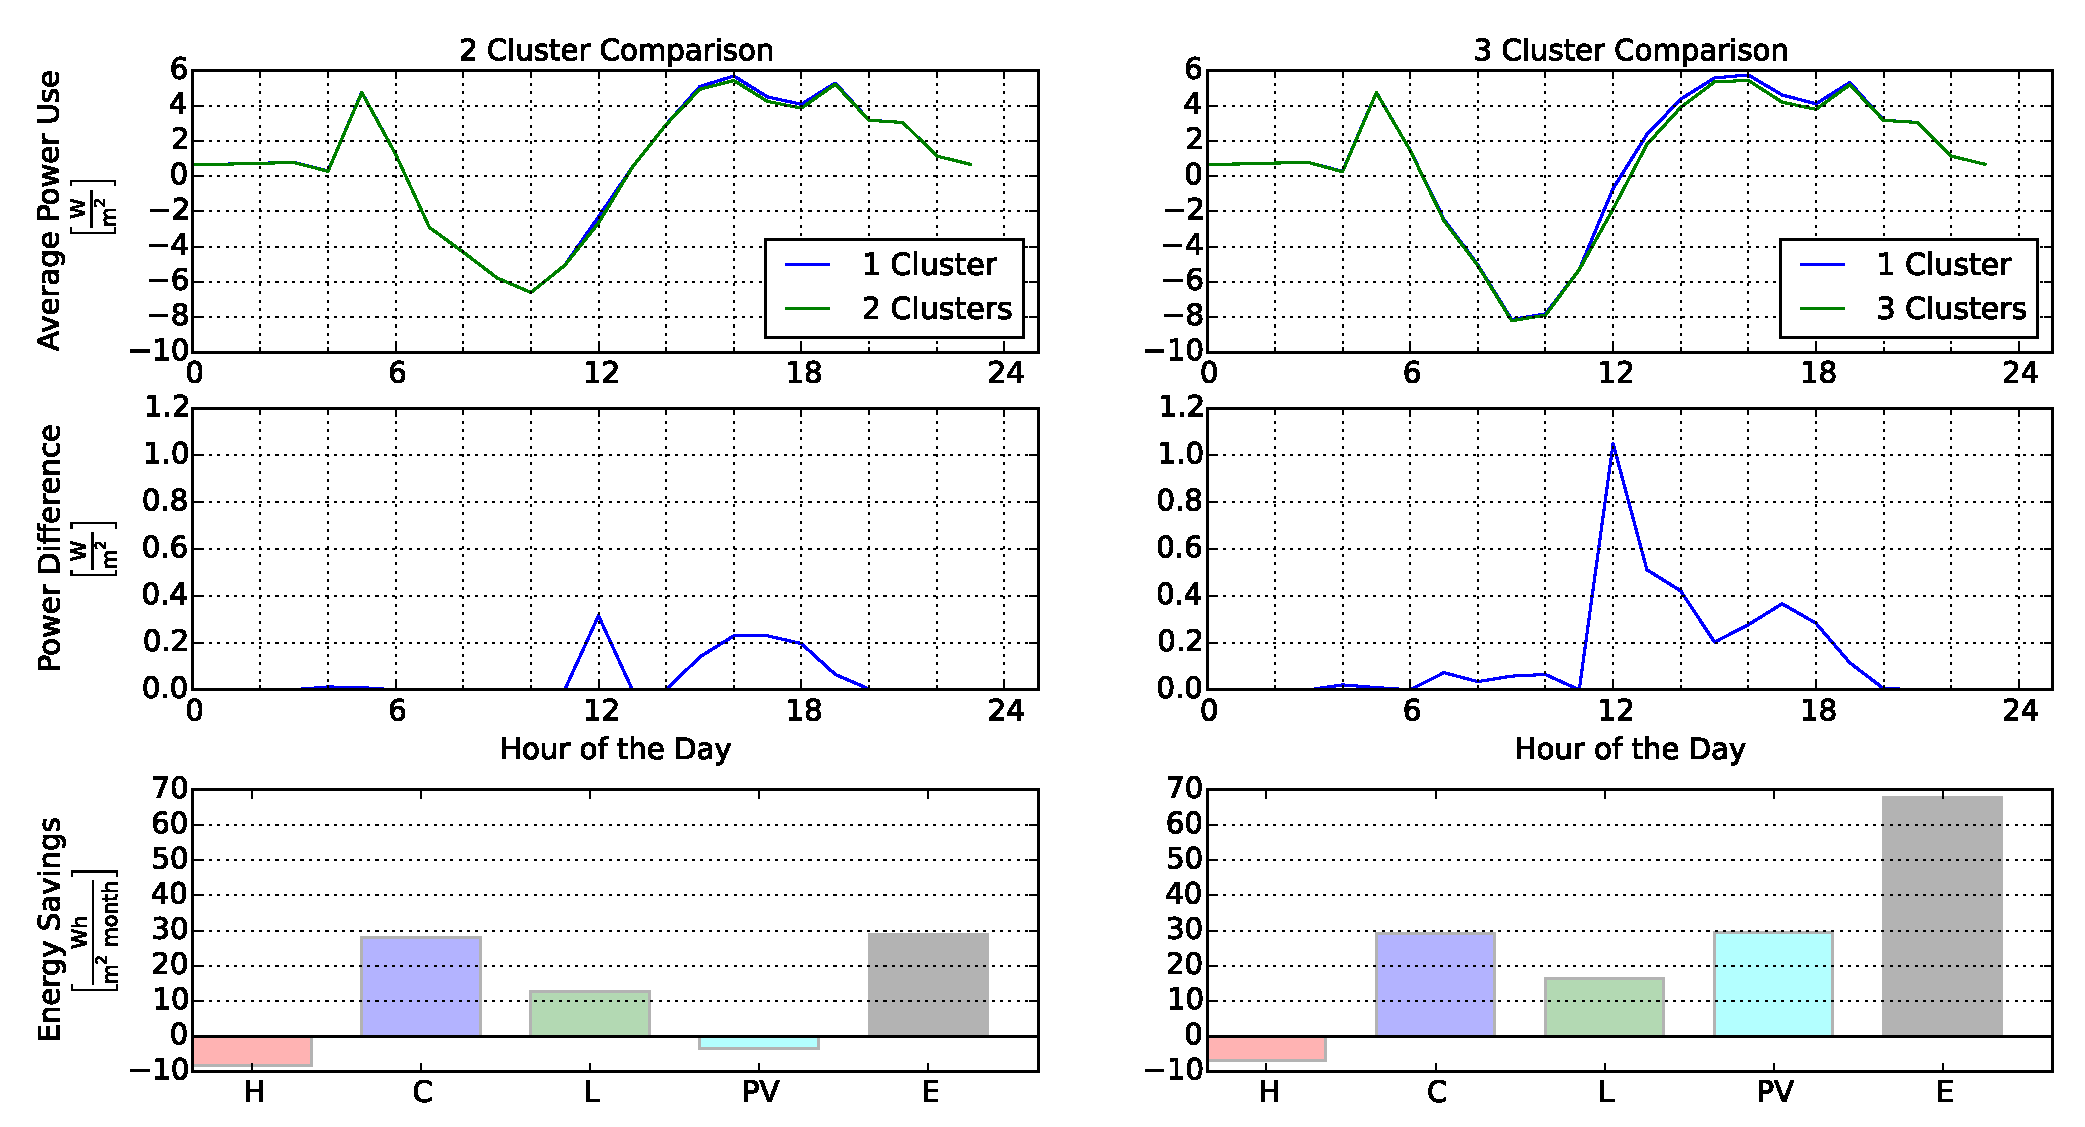
\includegraphics[width=\textwidth, trim= 0cm 0cm 0cm 0cm,clip]{cluster}
		\caption{Cluster analysis of the ASF. The left column details the analysis with 2 clusters, whereas the right column corresponds to the 3 cluster analysis. (a) shows the average power use per room area for the month of June, (b) details the corresponding power difference, and (c) visualizes the total energy savings, averaged for the months of March, June, September and December.}
		\label{fig:cluster}
		\end{center}
	\end{figure*}